\documentclass[11pt,a4paper]{article}

\usepackage[T1]{fontenc}
\usepackage[utf8]{inputenc}
\usepackage{lmodern}
\usepackage{textcomp}
% a true minus sign in text and in math (\textminus alone prints "=" in math mode; set at
% the start of the document, because hyperref redefines it there)
\AtBeginDocument{\DeclareRobustCommand{\textminus}{\ensuremath{-}}}
\usepackage[margin=2.5cm]{geometry}
\usepackage{amsmath,amssymb}
\usepackage{booktabs}
\usepackage{graphicx}
\usepackage{xcolor}
\usepackage[font=small,labelfont=bf]{caption}
\usepackage[authoryear,round]{natbib}
\usepackage{xr-hyper}
\usepackage[colorlinks=true,linkcolor=blue!50!black,citecolor=blue!50!black,urlcolor=blue!50!black]{hyperref}
\usepackage{microtype}
\usepackage{setspace}
% APA 7 citations: the reference list (bib_supplement.tex) is generated by analysis/apa_refs.py;
% two authors are joined by "and" in narrative and by "&" in parenthetical citations
\newif\ifapaparen
\DeclareRobustCommand{\apaand}{\ifapaparen\&\else and\fi}
\NewCommandCopy{\natcitep}{\citep}
\RenewDocumentCommand{\citep}{o o m}{{\apaparentrue%
  \IfNoValueTF{#1}{\natcitep{#3}}{\IfNoValueTF{#2}{\natcitep[#1]{#3}}{\natcitep[#1][#2]{#3}}}}}
\setstretch{1.08}
\emergencystretch=2em

% Every quoted result is a macro generated from the study's JSON outputs by
% analysis/make_tables.py, as in the main text. Licence: CC-BY 4.0 (see LICENSE).
\newcommand{\sh}{\ensuremath{\sharp}}
\newcommand{\flip}[1]{\textbf{#1}}
% AUTO-GENERATED by analysis/make_tables.py -- do not edit by hand.
\newcommand{\ratingTT}{1.953}
\newcommand{\ratingMsix}{2.477}
\newcommand{\nBelowTT}{4}
\newcommand{\gapClarCFourS}{\textminus{}3.4}
\newcommand{\gapClarCFourSmin}{+6.8}
\newcommand{\gapClarCFourV}{+39.8}
\newcommand{\gapClarCFourHK}{\textminus{}46.6}
\newcommand{\gapBassoonHK}{+55.0}
\newcommand{\gapHornV}{+198.1}
\newcommand{\shareInstrAll}{26}
\newcommand{\shareModelAll}{16}
\newcommand{\shareInterAll}{58}
\newcommand{\shareInstrLRAll}{34}
\newcommand{\shareModelLRAll}{18}
\newcommand{\shareInterLRAll}{48}
\newcommand{\signModelAll}{11/48}
\newcommand{\signModelPctAll}{23}
\newcommand{\signInstrAll}{45/112}
\newcommand{\signInstrPctAll}{40}
\newcommand{\medRangeModelsAll}{34.6}
\newcommand{\medRangeInstrAll}{97.7}
\newcommand{\shareInstrNoV}{55}
\newcommand{\shareModelNoV}{8}
\newcommand{\shareInterNoV}{36}
\newcommand{\shareInstrLRNoV}{56}
\newcommand{\shareModelLRNoV}{11}
\newcommand{\shareInterLRNoV}{33}
\newcommand{\signModelNoV}{6/24}
\newcommand{\signModelPctNoV}{25}
\newcommand{\signInstrNoV}{38/84}
\newcommand{\signInstrPctNoV}{45}
\newcommand{\medRangeModelsNoV}{20.0}
\newcommand{\medRangeInstrNoV}{93.8}
\newcommand{\shareInstrRegAll}{26}
\newcommand{\shareModelRegAll}{36}
\newcommand{\shareInterRegAll}{38}
\newcommand{\shareInstrLRRegAll}{25}
\newcommand{\shareModelLRRegAll}{44}
\newcommand{\shareInterLRRegAll}{31}
\newcommand{\signModelRegAll}{20/54}
\newcommand{\signModelPctRegAll}{37}
\newcommand{\signInstrRegAll}{44/144}
\newcommand{\signInstrPctRegAll}{31}
\newcommand{\medRangeModelsRegAll}{53.8}
\newcommand{\medRangeInstrRegAll}{70.8}
\newcommand{\shareInstrRegNoV}{43}
\newcommand{\shareModelRegNoV}{30}
\newcommand{\shareInterRegNoV}{27}
\newcommand{\shareInstrLRRegNoV}{39}
\newcommand{\shareModelLRRegNoV}{34}
\newcommand{\shareInterLRRegNoV}{28}
\newcommand{\signModelRegNoV}{10/27}
\newcommand{\signModelPctRegNoV}{37}
\newcommand{\signInstrRegNoV}{44/108}
\newcommand{\signInstrPctRegNoV}{41}
\newcommand{\medRangeModelsRegNoV}{18.0}
\newcommand{\medRangeInstrRegNoV}{58.3}
\newcommand{\rangeClarKernels}{86.4}
\newcommand{\rangeHKInstr}{101.6}
\newcommand{\sensKernelMed}{18.0}
\newcommand{\sensKernelMax}{76.0}
\newcommand{\sensRecordingMed}{6.0}
\newcommand{\sensRecordingMax}{31.5}
\newcommand{\sensExtractionMed}{0.4}
\newcommand{\sensExtractionMax}{2.8}
\newcommand{\sensCodecMed}{0.3}
\newcommand{\sensCodecMax}{1.2}
\newcommand{\sensIdealMed}{8.8}
\newcommand{\sensIdealMax}{19.1}
\newcommand{\sensABWideMed}{39.4}
\newcommand{\sensABWideMax}{129.8}
\newcommand{\sensABNarrowMed}{13.9}
\newcommand{\sensABNarrowMax}{41.1}
\newcommand{\sensInstrMed}{93.8}
\newcommand{\sensInstrMax}{101.6}
\newcommand{\sensVassExtractMax}{168.3}
\newcommand{\sensVassExtractMed}{9.3}
\newcommand{\codecWorstVass}{3.6}
\newcommand{\codecWorstStable}{0.9}
\newcommand{\extrVassWorst}{134.1}
\newcommand{\extrHKWorst}{2.8}
\newcommand{\hornVassLoose}{+64.0}
\newcommand{\idealHKFlat}{\textminus{}3.2}
\newcommand{\idealHKBase}{+4.6}
\newcommand{\iowaHKDThree}{\textminus{}22.1}
\newcommand{\philHKDThree}{\textminus{}30.8}
\newcommand{\diffHKDThree}{8.7}
\newcommand{\eoIowaDThree}{0.405}
\newcommand{\eoPhilDThree}{0.487}
\newcommand{\iowaHKCFour}{\textminus{}43.0}
\newcommand{\philHKCFour}{\textminus{}46.6}
\newcommand{\diffHKCFour}{3.6}
\newcommand{\eoIowaCFour}{0.194}
\newcommand{\eoPhilCFour}{0.178}
\newcommand{\iowaHKCFive}{\textminus{}11.7}
\newcommand{\philHKCFive}{\textminus{}43.2}
\newcommand{\diffHKCFive}{31.5}
\newcommand{\eoIowaCFive}{0.347}
\newcommand{\eoPhilCFive}{0.089}
\newcommand{\sethCFiveIowa}{\textminus{}7.4}
\newcommand{\sethCFivePhil}{+15.3}
\newcommand{\mechHKpairShare}{70}
\newcommand{\mechHKpairBeat}{62}
\newcommand{\mechHKpairFlo}{1304}
\newcommand{\mechHKpairFhi}{1242}
\newcommand{\mechSethFundShare}{36}
\newcommand{\mechSethFundBeat}{108}
\newcommand{\mechFundCBW}{1.49}
\newcommand{\mechFundERB}{1.84}
\newcommand{\mechHKTTovMsix}{0.53}
\newcommand{\mechCelloFundShare}{73}
\newcommand{\abStableWide}{7}
\newcommand{\abStableNarrow}{11}
\newcommand{\abNSpectra}{17}
\newcommand{\abUnstableNarrow}{cello C3, cello C4, French horn C4, oboe C4, oboe C5, piano C4}
\newcommand{\cutCelloCFour}{+3.7}
\newcommand{\gapCelloCFourHK}{\textminus{}1.7}
\newcommand{\gapHornHK}{\textminus{}0.6}
\newcommand{\clarHKExtrMax}{1.5}
\newcommand{\clarCutMaxRange}{1.8}
\newcommand{\abUnstableMaxAbs}{11.7}
\newcommand{\abClarPositiveCells}{Philharmonia D3: $a=0.35, b=1$; Iowa D3: $a=0.35, b=1$, $a=0.35, b=1.5$}
\newcommand{\mechFundMean}{315}
\newcommand{\mechFundGpct}{0.17}
\newcommand{\erbSignChanges}{cello C4, oboe C4}
\newcommand{\erbNSignChanges}{2}
\newcommand{\pianoB}{3.17}
\newcommand{\pianoBse}{6.3}
\newcommand{\pianoResid}{0.005}
\newcommand{\pianoTopRatio}{15.52}
\newcommand{\vassExpSignChanges}{3}
\newcommand{\vassExpNSpectra}{17}
\newcommand{\abGridA}{0.15, 0.2, 0.25, 0.3, 0.35}
\newcommand{\abGridB}{1.0, 1.5, 2.0, 2.5, 3.0}
\newcommand{\hkGapRaw}{0.233}
\newcommand{\hkGapZ}{0.120}
\newcommand{\hkGapMean}{0.085}
\newcommand{\dRBRawI}{0.049}
\newcommand{\pRBRawI}{$p<.001$}
\newcommand{\dRBRawH}{0.010}
\newcommand{\pRBRawH}{$p=.004$}
\newcommand{\dRBRawF}{0.147}
\newcommand{\pRBRawF}{$p<.001$}
\newcommand{\RfullBRaw}{0.674}
\newcommand{\dRBSizeI}{0.075}
\newcommand{\pRBSizeI}{$p<.001$}
\newcommand{\dRBSizeH}{0.037}
\newcommand{\pRBSizeH}{$p<.001$}
\newcommand{\dRBSizeF}{0.080}
\newcommand{\pRBSizeF}{$p<.001$}
\newcommand{\RfullBSize}{0.738}
\newcommand{\dRBRegI}{0.085}
\newcommand{\pRBRegI}{$p<.001$}
\newcommand{\dRBRegH}{0.042}
\newcommand{\pRBRegH}{$p<.001$}
\newcommand{\dRBRegF}{0.058}
\newcommand{\pRBRegF}{$p<.001$}
\newcommand{\RfullBReg}{0.749}
\newcommand{\dRBTrI}{0.074}
\newcommand{\pRBTrI}{$p<.001$}
\newcommand{\dRBTrH}{0.043}
\newcommand{\pRBTrH}{$p<.001$}
\newcommand{\dRBTrF}{0.082}
\newcommand{\pRBTrF}{$p<.001$}
\newcommand{\RfullBTr}{0.737}
\newcommand{\rHKBRaw}{0.713}
\newcommand{\rankHKBRaw}{4}
\newcommand{\rHuronBRaw}{0.685}
\newcommand{\rankHuronBRaw}{5}
\newcommand{\rSethBRaw}{0.393}
\newcommand{\rankSethBRaw}{14}
\newcommand{\rVassBRaw}{0.389}
\newcommand{\rankVassBRaw}{15}
\newcommand{\rCorpusBRaw}{0.722}
\newcommand{\rankCorpusBRaw}{3}
\newcommand{\rStolzBRaw}{0.740}
\newcommand{\rankStolzBRaw}{2}
\newcommand{\rCompositeBRaw}{0.801}
\newcommand{\rankCompositeBRaw}{1}
\newcommand{\rHKBSize}{0.761}
\newcommand{\rankHKBSize}{3}
\newcommand{\rHuronBSize}{0.692}
\newcommand{\rankHuronBSize}{5}
\newcommand{\rSethBSize}{0.521}
\newcommand{\rankSethBSize}{12}
\newcommand{\rVassBSize}{0.455}
\newcommand{\rankVassBSize}{14}
\newcommand{\rCorpusBSize}{0.719}
\newcommand{\rankCorpusBSize}{4}
\newcommand{\rStolzBSize}{0.794}
\newcommand{\rankStolzBSize}{2}
\newcommand{\rCompositeBSize}{0.856}
\newcommand{\rankCompositeBSize}{1}
\newcommand{\rHKBReg}{0.771}
\newcommand{\rankHKBReg}{3}
\newcommand{\rHuronBReg}{0.706}
\newcommand{\rankHuronBReg}{5}
\newcommand{\rSethBReg}{0.540}
\newcommand{\rankSethBReg}{11}
\newcommand{\rVassBReg}{0.477}
\newcommand{\rankVassBReg}{14}
\newcommand{\rCorpusBReg}{0.722}
\newcommand{\rankCorpusBReg}{4}
\newcommand{\rStolzBReg}{0.796}
\newcommand{\rankStolzBReg}{2}
\newcommand{\rCompositeBReg}{0.857}
\newcommand{\rankCompositeBReg}{1}
\newcommand{\rHKBTr}{0.751}
\newcommand{\rankHKBTr}{3}
\newcommand{\rHuronBTr}{0.692}
\newcommand{\rankHuronBTr}{5}
\newcommand{\rSethBTr}{0.540}
\newcommand{\rankSethBTr}{12}
\newcommand{\rVassBTr}{0.453}
\newcommand{\rankVassBTr}{14}
\newcommand{\rCorpusBTr}{0.719}
\newcommand{\rankCorpusBTr}{4}
\newcommand{\rStolzBTr}{0.794}
\newcommand{\rankStolzBTr}{2}
\newcommand{\rCompositeBTr}{0.855}
\newcommand{\rankCompositeBTr}{1}
\newcommand{\dRJRawI}{0.005}
\newcommand{\pRJRawI}{$p=.344$}
\newcommand{\dRJRawH}{0.042}
\newcommand{\pRJRawH}{$p=.009$}
\newcommand{\dRJRawF}{0.141}
\newcommand{\pRJRawF}{$p<.001$}
\newcommand{\RfullJRaw}{0.414}
\newcommand{\dRJSizeI}{0.033}
\newcommand{\pRJSizeI}{$p=.013$}
\newcommand{\dRJSizeH}{0.100}
\newcommand{\pRJSizeH}{$p<.001$}
\newcommand{\dRJSizeF}{0.045}
\newcommand{\pRJSizeF}{$p=.004$}
\newcommand{\RfullJSize}{0.500}
\newcommand{\dRJRegI}{0.026}
\newcommand{\pRJRegI}{$p=.025$}
\newcommand{\dRJRegH}{0.108}
\newcommand{\pRJRegH}{$p<.001$}
\newcommand{\dRJRegF}{0.033}
\newcommand{\pRJRegF}{$p=.011$}
\newcommand{\RfullJReg}{0.516}
\newcommand{\dRJTrI}{0.068}
\newcommand{\pRJTrI}{$p<.001$}
\newcommand{\dRJTrH}{0.090}
\newcommand{\pRJTrH}{$p<.001$}
\newcommand{\dRJTrF}{0.031}
\newcommand{\pRJTrF}{$p=.012$}
\newcommand{\RfullJTr}{0.534}
\newcommand{\rHKJRaw}{0.440}
\newcommand{\rankHKJRaw}{8}
\newcommand{\rHuronJRaw}{0.680}
\newcommand{\rankHuronJRaw}{3}
\newcommand{\rSethJRaw}{0.065}
\newcommand{\rankSethJRaw}{13}
\newcommand{\rVassJRaw}{0.042}
\newcommand{\rankVassJRaw}{15}
\newcommand{\rCorpusJRaw}{0.568}
\newcommand{\rankCorpusJRaw}{5}
\newcommand{\rStolzJRaw}{0.723}
\newcommand{\rankStolzJRaw}{1}
\newcommand{\rCompositeJRaw}{0.628}
\newcommand{\rankCompositeJRaw}{4}
\newcommand{\rHKJSize}{0.529}
\newcommand{\rankHKJSize}{8}
\newcommand{\rHuronJSize}{0.682}
\newcommand{\rankHuronJSize}{4}
\newcommand{\rSethJSize}{0.171}
\newcommand{\rankSethJSize}{13}
\newcommand{\rVassJSize}{0.087}
\newcommand{\rankVassJSize}{14}
\newcommand{\rCorpusJSize}{0.568}
\newcommand{\rankCorpusJSize}{6}
\newcommand{\rStolzJSize}{0.783}
\newcommand{\rankStolzJSize}{1}
\newcommand{\rCompositeJSize}{0.694}
\newcommand{\rankCompositeJSize}{3}
\newcommand{\rHKJReg}{0.500}
\newcommand{\rankHKJReg}{9}
\newcommand{\rHuronJReg}{0.676}
\newcommand{\rankHuronJReg}{3}
\newcommand{\rSethJReg}{0.172}
\newcommand{\rankSethJReg}{12}
\newcommand{\rVassJReg}{0.026}
\newcommand{\rankVassJReg}{14}
\newcommand{\rCorpusJReg}{0.537}
\newcommand{\rankCorpusJReg}{7}
\newcommand{\rStolzJReg}{0.765}
\newcommand{\rankStolzJReg}{1}
\newcommand{\rCompositeJReg}{0.674}
\newcommand{\rankCompositeJReg}{4}
\newcommand{\rHKJTr}{0.594}
\newcommand{\rankHKJTr}{6}
\newcommand{\rHuronJTr}{0.682}
\newcommand{\rankHuronJTr}{4}
\newcommand{\rSethJTr}{0.428}
\newcommand{\rankSethJTr}{12}
\newcommand{\rVassJTr}{0.222}
\newcommand{\rankVassJTr}{13}
\newcommand{\rCorpusJTr}{0.568}
\newcommand{\rankCorpusJTr}{7}
\newcommand{\rStolzJTr}{0.783}
\newcommand{\rankStolzJTr}{1}
\newcommand{\rCompositeJTr}{0.716}
\newcommand{\rankCompositeJTr}{3}
\newcommand{\ratioFamIntBRaw}{3.0}
\newcommand{\ratioFamIntJRaw}{26}
\newcommand{\nHarm}{160}
\newcommand{\ntrialsHarm}{7{,}440}
\newcommand{\gapObsHarm}{+0.19}
\newcommand{\gapObsHarmCI}{[+0.04, +0.35]}
\newcommand{\gapHKHarm}{+0.18}
\newcommand{\gapHKHarmCI}{[+0.03, +0.33]}
\newcommand{\gapHKHHarm}{+0.12}
\newcommand{\gapHKHHarmCI}{[\textminus{}0.03, +0.28]}
\newcommand{\gapCompHarm}{+0.16}
\newcommand{\gapCompHarmCI}{[+0.01, +0.31]}
\newcommand{\gapSethHarm}{+0.18}
\newcommand{\gapSethHarmCI}{[+0.03, +0.33]}
\newcommand{\gapHHarm}{+0.10}
\newcommand{\gapHHarmCI}{[\textminus{}0.04, +0.26]}
\newcommand{\dipObsHarm}{+0.38}
\newcommand{\dipObsHarmCI}{[+0.25, +0.51]}
\newcommand{\dipHKHarm}{+0.29}
\newcommand{\dipHKHarmCI}{[+0.17, +0.42]}
\newcommand{\dipHKHHarm}{+0.10}
\newcommand{\dipHKHHarmCI}{[\textminus{}0.02, +0.22]}
\newcommand{\dipCompHarm}{+0.15}
\newcommand{\dipCompHarmCI}{[+0.03, +0.27]}
\newcommand{\dipSethHarm}{+0.34}
\newcommand{\dipSethHarmCI}{[+0.22, +0.47]}
\newcommand{\dipHHarm}{+0.08}
\newcommand{\dipHHarmCI}{[\textminus{}0.03, +0.19]}
\newcommand{\shareHKHarm}{5}
\newcommand{\rfitHKHarm}{0.22}
\newcommand{\shareHKHHarm}{38}
\newcommand{\rfitHKHHarm}{0.37}
\newcommand{\shareCompHarm}{17}
\newcommand{\rfitCompHarm}{0.35}
\newcommand{\shareHHarm}{46}
\newcommand{\rfitHHarm}{0.33}
\newcommand{\rawsdHarm}{1.31}
\newcommand{\nEqfive}{147}
\newcommand{\ntrialsEqfive}{11{,}754}
\newcommand{\gapObsEqfive}{+0.18}
\newcommand{\gapObsEqfiveCI}{[+0.07, +0.30]}
\newcommand{\gapHKEqfive}{+0.19}
\newcommand{\gapHKEqfiveCI}{[+0.07, +0.31]}
\newcommand{\gapHKHEqfive}{+0.04}
\newcommand{\gapHKHEqfiveCI}{[\textminus{}0.08, +0.16]}
\newcommand{\gapCompEqfive}{+0.05}
\newcommand{\gapCompEqfiveCI}{[\textminus{}0.06, +0.16]}
\newcommand{\gapSethEqfive}{+0.16}
\newcommand{\gapSethEqfiveCI}{[+0.05, +0.28]}
\newcommand{\gapHEqfive}{\textminus{}0.04}
\newcommand{\gapHEqfiveCI}{[\textminus{}0.16, +0.07]}
\newcommand{\dipObsEqfive}{+0.27}
\newcommand{\dipObsEqfiveCI}{[+0.14, +0.40]}
\newcommand{\dipHKEqfive}{+0.12}
\newcommand{\dipHKEqfiveCI}{[\textminus{}0.02, +0.24]}
\newcommand{\dipHKHEqfive}{\textminus{}0.09}
\newcommand{\dipHKHEqfiveCI}{[\textminus{}0.21, +0.04]}
\newcommand{\dipCompEqfive}{\textminus{}0.13}
\newcommand{\dipCompEqfiveCI}{[\textminus{}0.26, \textminus{}0.01]}
\newcommand{\dipSethEqfive}{+0.16}
\newcommand{\dipSethEqfiveCI}{[+0.03, +0.29]}
\newcommand{\dipHEqfive}{\textminus{}0.11}
\newcommand{\dipHEqfiveCI}{[\textminus{}0.23, +0.02]}
\newcommand{\shareHKEqfive}{-2}
\newcommand{\rfitHKEqfive}{0.52}
\newcommand{\shareHKHEqfive}{76}
\newcommand{\rfitHKHEqfive}{0.65}
\newcommand{\shareCompEqfive}{73}
\newcommand{\rfitCompEqfive}{0.69}
\newcommand{\shareHEqfive}{123}
\newcommand{\rfitHEqfive}{0.41}
\newcommand{\rawsdEqfive}{1.35}
\newcommand{\nNothree}{151}
\newcommand{\ntrialsNothree}{12{,}000}
\newcommand{\gapObsNothree}{+0.16}
\newcommand{\gapObsNothreeCI}{[+0.06, +0.26]}
\newcommand{\gapHKNothree}{+0.15}
\newcommand{\gapHKNothreeCI}{[+0.05, +0.25]}
\newcommand{\gapHKHNothree}{+0.01}
\newcommand{\gapHKHNothreeCI}{[\textminus{}0.10, +0.12]}
\newcommand{\gapCompNothree}{0.00}
\newcommand{\gapCompNothreeCI}{[\textminus{}0.10, +0.10]}
\newcommand{\gapSethNothree}{+0.13}
\newcommand{\gapSethNothreeCI}{[+0.03, +0.23]}
\newcommand{\gapHNothree}{\textminus{}0.08}
\newcommand{\gapHNothreeCI}{[\textminus{}0.18, +0.03]}
\newcommand{\dipObsNothree}{+0.23}
\newcommand{\dipObsNothreeCI}{[+0.14, +0.33]}
\newcommand{\dipHKNothree}{+0.28}
\newcommand{\dipHKNothreeCI}{[+0.19, +0.38]}
\newcommand{\dipHKHNothree}{+0.23}
\newcommand{\dipHKHNothreeCI}{[+0.14, +0.32]}
\newcommand{\dipCompNothree}{+0.21}
\newcommand{\dipCompNothreeCI}{[+0.12, +0.31]}
\newcommand{\dipSethNothree}{+0.28}
\newcommand{\dipSethNothreeCI}{[+0.18, +0.38]}
\newcommand{\dipHNothree}{+0.16}
\newcommand{\dipHNothreeCI}{[+0.07, +0.25]}
\newcommand{\shareHKNothree}{9}
\newcommand{\rfitHKNothree}{0.59}
\newcommand{\shareHKHNothree}{96}
\newcommand{\rfitHKHNothree}{0.70}
\newcommand{\shareCompNothree}{102}
\newcommand{\rfitCompNothree}{0.66}
\newcommand{\shareHNothree}{147}
\newcommand{\rfitHNothree}{0.33}
\newcommand{\rawsdNothree}{1.34}
\newcommand{\nFlute}{188}
\newcommand{\ntrialsFlute}{7{,}500}
\newcommand{\gapObsFlute}{+0.35}
\newcommand{\gapObsFluteCI}{[+0.22, +0.48]}
\newcommand{\gapHKFlute}{+0.36}
\newcommand{\gapHKFluteCI}{[+0.23, +0.50]}
\newcommand{\gapHKHFlute}{+0.34}
\newcommand{\gapHKHFluteCI}{[+0.20, +0.47]}
\newcommand{\gapCompFlute}{+0.27}
\newcommand{\gapCompFluteCI}{[+0.13, +0.40]}
\newcommand{\gapSethFlute}{+0.39}
\newcommand{\gapSethFluteCI}{[+0.26, +0.53]}
\newcommand{\gapHFlute}{+0.21}
\newcommand{\gapHFluteCI}{[+0.08, +0.35]}
\newcommand{\dipObsFlute}{+0.23}
\newcommand{\dipObsFluteCI}{[+0.11, +0.34]}
\newcommand{\dipHKFlute}{+0.10}
\newcommand{\dipHKFluteCI}{[\textminus{}0.02, +0.22]}
\newcommand{\dipHKHFlute}{+0.03}
\newcommand{\dipHKHFluteCI}{[\textminus{}0.09, +0.15]}
\newcommand{\dipCompFlute}{\textminus{}0.19}
\newcommand{\dipCompFluteCI}{[\textminus{}0.31, \textminus{}0.08]}
\newcommand{\dipSethFlute}{+0.14}
\newcommand{\dipSethFluteCI}{[+0.02, +0.25]}
\newcommand{\dipHFlute}{\textminus{}0.15}
\newcommand{\dipHFluteCI}{[\textminus{}0.27, \textminus{}0.03]}
\newcommand{\shareHKFlute}{-5}
\newcommand{\rfitHKFlute}{0.74}
\newcommand{\shareHKHFlute}{3}
\newcommand{\rfitHKHFlute}{0.75}
\newcommand{\shareCompFlute}{23}
\newcommand{\rfitCompFlute}{0.60}
\newcommand{\shareHFlute}{38}
\newcommand{\rfitHFlute}{0.21}
\newcommand{\rawsdFlute}{1.14}
\newcommand{\nGuitar}{186}
\newcommand{\ntrialsGuitar}{7{,}379}
\newcommand{\gapObsGuitar}{+0.39}
\newcommand{\gapObsGuitarCI}{[+0.25, +0.55]}
\newcommand{\gapHKGuitar}{+0.40}
\newcommand{\gapHKGuitarCI}{[+0.25, +0.55]}
\newcommand{\gapHKHGuitar}{+0.37}
\newcommand{\gapHKHGuitarCI}{[+0.23, +0.52]}
\newcommand{\gapCompGuitar}{+0.33}
\newcommand{\gapCompGuitarCI}{[+0.19, +0.48]}
\newcommand{\gapSethGuitar}{+0.38}
\newcommand{\gapSethGuitarCI}{[+0.24, +0.54]}
\newcommand{\gapHGuitar}{+0.30}
\newcommand{\gapHGuitarCI}{[+0.16, +0.44]}
\newcommand{\dipObsGuitar}{+0.33}
\newcommand{\dipObsGuitarCI}{[+0.20, +0.46]}
\newcommand{\dipHKGuitar}{+0.32}
\newcommand{\dipHKGuitarCI}{[+0.19, +0.45]}
\newcommand{\dipHKHGuitar}{+0.25}
\newcommand{\dipHKHGuitarCI}{[+0.12, +0.39]}
\newcommand{\dipCompGuitar}{+0.14}
\newcommand{\dipCompGuitarCI}{[+0.01, +0.27]}
\newcommand{\dipSethGuitar}{+0.35}
\newcommand{\dipSethGuitarCI}{[+0.22, +0.48]}
\newcommand{\dipHGuitar}{+0.09}
\newcommand{\dipHGuitarCI}{[\textminus{}0.04, +0.21]}
\newcommand{\shareHKGuitar}{-1}
\newcommand{\rfitHKGuitar}{0.86}
\newcommand{\shareHKHGuitar}{6}
\newcommand{\rfitHKHGuitar}{0.88}
\newcommand{\shareCompGuitar}{16}
\newcommand{\rfitCompGuitar}{0.69}
\newcommand{\shareHGuitar}{25}
\newcommand{\rfitHGuitar}{0.26}
\newcommand{\rawsdGuitar}{1.16}
\newcommand{\nPiano}{191}
\newcommand{\ntrialsPiano}{7{,}382}
\newcommand{\gapObsPiano}{+0.33}
\newcommand{\gapObsPianoCI}{[+0.18, +0.48]}
\newcommand{\gapHKPiano}{+0.32}
\newcommand{\gapHKPianoCI}{[+0.18, +0.48]}
\newcommand{\gapHKHPiano}{+0.29}
\newcommand{\gapHKHPianoCI}{[+0.15, +0.45]}
\newcommand{\gapCompPiano}{+0.25}
\newcommand{\gapCompPianoCI}{[+0.11, +0.40]}
\newcommand{\gapSethPiano}{+0.30}
\newcommand{\gapSethPianoCI}{[+0.16, +0.45]}
\newcommand{\gapHPiano}{+0.22}
\newcommand{\gapHPianoCI}{[+0.08, +0.37]}
\newcommand{\dipObsPiano}{+0.39}
\newcommand{\dipObsPianoCI}{[+0.27, +0.51]}
\newcommand{\dipHKPiano}{+0.36}
\newcommand{\dipHKPianoCI}{[+0.24, +0.48]}
\newcommand{\dipHKHPiano}{+0.28}
\newcommand{\dipHKHPianoCI}{[+0.17, +0.41]}
\newcommand{\dipCompPiano}{+0.13}
\newcommand{\dipCompPianoCI}{[+0.01, +0.25]}
\newcommand{\dipSethPiano}{+0.39}
\newcommand{\dipSethPianoCI}{[+0.28, +0.51]}
\newcommand{\dipHPiano}{+0.10}
\newcommand{\dipHPianoCI}{[\textminus{}0.02, +0.22]}
\newcommand{\shareHKPiano}{1}
\newcommand{\rfitHKPiano}{0.88}
\newcommand{\shareHKHPiano}{9}
\newcommand{\rfitHKHPiano}{0.90}
\newcommand{\shareCompPiano}{23}
\newcommand{\rfitCompPiano}{0.70}
\newcommand{\shareHPiano}{33}
\newcommand{\rfitHPiano}{0.27}
\newcommand{\rawsdPiano}{1.16}
\newcommand{\nPure}{151}
\newcommand{\ntrialsPure}{7{,}397}
\newcommand{\gapObsPure}{+0.21}
\newcommand{\gapObsPureCI}{[+0.08, +0.34]}
\newcommand{\gapHKPure}{+0.21}
\newcommand{\gapHKPureCI}{[+0.08, +0.34]}
\newcommand{\gapHKHPure}{+0.18}
\newcommand{\gapHKHPureCI}{[+0.05, +0.31]}
\newcommand{\gapCompPure}{+0.14}
\newcommand{\gapCompPureCI}{[+0.02, +0.26]}
\newcommand{\gapSethPure}{+0.15}
\newcommand{\gapSethPureCI}{[+0.03, +0.27]}
\newcommand{\gapHPure}{+0.15}
\newcommand{\gapHPureCI}{[+0.02, +0.27]}
\newcommand{\dipObsPure}{+0.28}
\newcommand{\dipObsPureCI}{[+0.17, +0.39]}
\newcommand{\dipHKPure}{+0.28}
\newcommand{\dipHKPureCI}{[+0.17, +0.39]}
\newcommand{\dipHKHPure}{+0.20}
\newcommand{\dipHKHPureCI}{[+0.10, +0.32]}
\newcommand{\dipCompPure}{+0.10}
\newcommand{\dipCompPureCI}{[\textminus{}0.01, +0.22]}
\newcommand{\dipSethPure}{+0.29}
\newcommand{\dipSethPureCI}{[+0.18, +0.41]}
\newcommand{\dipHPure}{+0.11}
\newcommand{\dipHPureCI}{[+0.01, +0.23]}
\newcommand{\shareHKPure}{0}
\newcommand{\rfitHKPure}{0.79}
\newcommand{\shareHKHPure}{13}
\newcommand{\rfitHKHPure}{0.82}
\newcommand{\shareCompPure}{32}
\newcommand{\rfitCompPure}{0.74}
\newcommand{\shareHPure}{30}
\newcommand{\rfitHPure}{0.15}
\newcommand{\rawsdPure}{1.23}
\newcommand{\nBonang}{146}
\newcommand{\ntrialsBonang}{7{,}247}
\newcommand{\gapObsBonang}{+0.38}
\newcommand{\gapObsBonangCI}{[+0.22, +0.53]}
\newcommand{\gapHKBonang}{+0.29}
\newcommand{\gapHKBonangCI}{[+0.14, +0.44]}
\newcommand{\gapHKHBonang}{+0.31}
\newcommand{\gapHKHBonangCI}{[+0.16, +0.46]}
\newcommand{\gapCompBonang}{+0.28}
\newcommand{\gapCompBonangCI}{[+0.12, +0.42]}
\newcommand{\gapSethBonang}{+0.35}
\newcommand{\gapSethBonangCI}{[+0.20, +0.50]}
\newcommand{\gapHBonang}{+0.32}
\newcommand{\gapHBonangCI}{[+0.16, +0.47]}
\newcommand{\dipObsBonang}{+0.36}
\newcommand{\dipObsBonangCI}{[+0.23, +0.49]}
\newcommand{\dipHKBonang}{+0.30}
\newcommand{\dipHKBonangCI}{[+0.18, +0.42]}
\newcommand{\dipHKHBonang}{+0.04}
\newcommand{\dipHKHBonangCI}{[\textminus{}0.09, +0.17]}
\newcommand{\dipCompBonang}{+0.13}
\newcommand{\dipCompBonangCI}{[+0.01, +0.25]}
\newcommand{\dipSethBonang}{+0.35}
\newcommand{\dipSethBonangCI}{[+0.22, +0.47]}
\newcommand{\dipHBonang}{+0.04}
\newcommand{\dipHBonangCI}{[\textminus{}0.08, +0.16]}
\newcommand{\shareHKBonang}{24}
\newcommand{\rfitHKBonang}{0.12}
\newcommand{\shareHKHBonang}{19}
\newcommand{\rfitHKHBonang}{0.30}
\newcommand{\shareCompBonang}{27}
\newcommand{\rfitCompBonang}{0.31}
\newcommand{\shareHBonang}{16}
\newcommand{\rfitHBonang}{0.30}
\newcommand{\rawsdBonang}{1.20}
\newcommand{\nStr}{153}
\newcommand{\ntrialsStr}{7{,}443}
\newcommand{\gapObsStr}{\textminus{}0.02}
\newcommand{\gapObsStrCI}{[\textminus{}0.17, +0.11]}
\newcommand{\gapHKStr}{\textminus{}0.02}
\newcommand{\gapHKStrCI}{[\textminus{}0.17, +0.11]}
\newcommand{\gapHKHStr}{\textminus{}0.02}
\newcommand{\gapHKHStrCI}{[\textminus{}0.17, +0.11]}
\newcommand{\gapCompStr}{\textminus{}0.02}
\newcommand{\gapCompStrCI}{[\textminus{}0.16, +0.12]}
\newcommand{\gapSethStr}{\textminus{}0.04}
\newcommand{\gapSethStrCI}{[\textminus{}0.18, +0.10]}
\newcommand{\gapHStr}{\textminus{}0.02}
\newcommand{\gapHStrCI}{[\textminus{}0.17, +0.11]}
\newcommand{\dipObsStr}{\textminus{}0.03}
\newcommand{\dipObsStrCI}{[\textminus{}0.15, +0.09]}
\newcommand{\dipHKStr}{\textminus{}0.03}
\newcommand{\dipHKStrCI}{[\textminus{}0.15, +0.08]}
\newcommand{\dipHKHStr}{\textminus{}0.03}
\newcommand{\dipHKHStrCI}{[\textminus{}0.15, +0.08]}
\newcommand{\dipCompStr}{\textminus{}0.04}
\newcommand{\dipCompStrCI}{[\textminus{}0.15, +0.08]}
\newcommand{\dipSethStr}{\textminus{}0.03}
\newcommand{\dipSethStrCI}{[\textminus{}0.15, +0.08]}
\newcommand{\dipHStr}{\textminus{}0.03}
\newcommand{\dipHStrCI}{[\textminus{}0.15, +0.09]}
\newcommand{\shareHKStr}{-16}
\newcommand{\rfitHKStr}{0.42}
\newcommand{\shareHKHStr}{-4}
\newcommand{\rfitHKHStr}{0.43}
\newcommand{\shareCompStr}{27}
\newcommand{\rfitCompStr}{0.38}
\newcommand{\shareHStr}{-3}
\newcommand{\rfitHStr}{0.00}
\newcommand{\rawsdStr}{1.29}
\newcommand{\nComp}{154}
\newcommand{\ntrialsComp}{7{,}398}
\newcommand{\gapObsComp}{+0.02}
\newcommand{\gapObsCompCI}{[\textminus{}0.12, +0.14]}
\newcommand{\gapHKComp}{\textminus{}0.02}
\newcommand{\gapHKCompCI}{[\textminus{}0.15, +0.10]}
\newcommand{\gapHKHComp}{\textminus{}0.02}
\newcommand{\gapHKHCompCI}{[\textminus{}0.15, +0.11]}
\newcommand{\gapCompComp}{\textminus{}0.04}
\newcommand{\gapCompCompCI}{[\textminus{}0.17, +0.08]}
\newcommand{\gapSethComp}{0.00}
\newcommand{\gapSethCompCI}{[\textminus{}0.13, +0.12]}
\newcommand{\gapHComp}{+0.03}
\newcommand{\gapHCompCI}{[\textminus{}0.11, +0.15]}
\newcommand{\dipObsComp}{+0.03}
\newcommand{\dipObsCompCI}{[\textminus{}0.09, +0.14]}
\newcommand{\dipHKComp}{+0.03}
\newcommand{\dipHKCompCI}{[\textminus{}0.09, +0.14]}
\newcommand{\dipHKHComp}{+0.03}
\newcommand{\dipHKHCompCI}{[\textminus{}0.08, +0.15]}
\newcommand{\dipCompComp}{+0.02}
\newcommand{\dipCompCompCI}{[\textminus{}0.09, +0.13]}
\newcommand{\dipSethComp}{+0.03}
\newcommand{\dipSethCompCI}{[\textminus{}0.08, +0.14]}
\newcommand{\dipHComp}{+0.04}
\newcommand{\dipHCompCI}{[\textminus{}0.07, +0.16]}
\newcommand{\shareHKComp}{218}
\newcommand{\rfitHKComp}{0.39}
\newcommand{\shareHKHComp}{194}
\newcommand{\rfitHKHComp}{0.39}
\newcommand{\shareCompComp}{321}
\newcommand{\rfitCompComp}{0.37}
\newcommand{\shareHComp}{-39}
\newcommand{\rfitHComp}{0.03}
\newcommand{\rawsdComp}{1.20}
\newcommand{\nHarmKr}{40}
\newcommand{\ntrialsHarmKr}{4{,}187}
\newcommand{\gapObsHarmKr}{+0.07}
\newcommand{\gapObsHarmKrCI}{[\textminus{}0.12, +0.25]}
\newcommand{\gapHKHarmKr}{+0.06}
\newcommand{\gapHKHarmKrCI}{[\textminus{}0.12, +0.24]}
\newcommand{\gapHKHHarmKr}{\textminus{}0.03}
\newcommand{\gapHKHHarmKrCI}{[\textminus{}0.20, +0.14]}
\newcommand{\gapCompHarmKr}{+0.03}
\newcommand{\gapCompHarmKrCI}{[\textminus{}0.14, +0.21]}
\newcommand{\gapSethHarmKr}{+0.07}
\newcommand{\gapSethHarmKrCI}{[\textminus{}0.11, +0.25]}
\newcommand{\gapHHarmKr}{\textminus{}0.03}
\newcommand{\gapHHarmKrCI}{[\textminus{}0.20, +0.13]}
\newcommand{\dipObsHarmKr}{+0.25}
\newcommand{\dipObsHarmKrCI}{[+0.10, +0.42]}
\newcommand{\dipHKHarmKr}{+0.19}
\newcommand{\dipHKHarmKrCI}{[+0.05, +0.35]}
\newcommand{\dipHKHHarmKr}{\textminus{}0.04}
\newcommand{\dipHKHHarmKrCI}{[\textminus{}0.17, +0.09]}
\newcommand{\dipCompHarmKr}{+0.07}
\newcommand{\dipCompHarmKrCI}{[\textminus{}0.08, +0.21]}
\newcommand{\dipSethHarmKr}{+0.26}
\newcommand{\dipSethHarmKrCI}{[+0.11, +0.42]}
\newcommand{\dipHHarmKr}{\textminus{}0.04}
\newcommand{\dipHHarmKrCI}{[\textminus{}0.18, +0.09]}
\newcommand{\shareHKHarmKr}{11}
\newcommand{\rfitHKHarmKr}{0.05}
\newcommand{\shareHKHHarmKr}{140}
\newcommand{\rfitHKHHarmKr}{0.14}
\newcommand{\shareCompHarmKr}{49}
\newcommand{\rfitCompHarmKr}{0.10}
\newcommand{\shareHHarmKr}{144}
\newcommand{\rfitHHarmKr}{0.14}
\newcommand{\rawsdHarmKr}{1.00}
\newcommand{\nStrKr}{37}
\newcommand{\ntrialsStrKr}{3{,}961}
\newcommand{\gapObsStrKr}{\textminus{}0.17}
\newcommand{\gapObsStrKrCI}{[\textminus{}0.34, 0.00]}
\newcommand{\gapHKStrKr}{\textminus{}0.17}
\newcommand{\gapHKStrKrCI}{[\textminus{}0.34, 0.00]}
\newcommand{\gapHKHStrKr}{\textminus{}0.18}
\newcommand{\gapHKHStrKrCI}{[\textminus{}0.34, 0.00]}
\newcommand{\gapCompStrKr}{\textminus{}0.17}
\newcommand{\gapCompStrKrCI}{[\textminus{}0.34, 0.00]}
\newcommand{\gapSethStrKr}{\textminus{}0.14}
\newcommand{\gapSethStrKrCI}{[\textminus{}0.30, +0.03]}
\newcommand{\gapHStrKr}{\textminus{}0.18}
\newcommand{\gapHStrKrCI}{[\textminus{}0.34, 0.00]}
\newcommand{\dipObsStrKr}{\textminus{}0.06}
\newcommand{\dipObsStrKrCI}{[\textminus{}0.21, +0.10]}
\newcommand{\dipHKStrKr}{\textminus{}0.06}
\newcommand{\dipHKStrKrCI}{[\textminus{}0.21, +0.10]}
\newcommand{\dipHKHStrKr}{\textminus{}0.06}
\newcommand{\dipHKHStrKrCI}{[\textminus{}0.21, +0.10]}
\newcommand{\dipCompStrKr}{\textminus{}0.06}
\newcommand{\dipCompStrKrCI}{[\textminus{}0.21, +0.10]}
\newcommand{\dipSethStrKr}{\textminus{}0.05}
\newcommand{\dipSethStrKrCI}{[\textminus{}0.21, +0.11]}
\newcommand{\dipHStrKr}{\textminus{}0.06}
\newcommand{\dipHStrKrCI}{[\textminus{}0.21, +0.11]}
\newcommand{\shareHKStrKr}{0}
\newcommand{\rfitHKStrKr}{0.00}
\newcommand{\shareHKHStrKr}{-3}
\newcommand{\rfitHKHStrKr}{0.00}
\newcommand{\shareCompStrKr}{-0}
\newcommand{\rfitCompStrKr}{0.00}
\newcommand{\shareHStrKr}{-3}
\newcommand{\rfitHStrKr}{0.00}
\newcommand{\rawsdStrKr}{1.00}
\newcommand{\nCompKr}{45}
\newcommand{\ntrialsCompKr}{4{,}777}
\newcommand{\gapObsCompKr}{\textminus{}0.21}
\newcommand{\gapObsCompKrCI}{[\textminus{}0.39, \textminus{}0.04]}
\newcommand{\gapHKCompKr}{\textminus{}0.18}
\newcommand{\gapHKCompKrCI}{[\textminus{}0.35, \textminus{}0.02]}
\newcommand{\gapHKHCompKr}{\textminus{}0.14}
\newcommand{\gapHKHCompKrCI}{[\textminus{}0.31, +0.03]}
\newcommand{\gapCompCompKr}{\textminus{}0.16}
\newcommand{\gapCompCompKrCI}{[\textminus{}0.33, 0.00]}
\newcommand{\gapSethCompKr}{\textminus{}0.16}
\newcommand{\gapSethCompKrCI}{[\textminus{}0.33, +0.01]}
\newcommand{\gapHCompKr}{\textminus{}0.19}
\newcommand{\gapHCompKrCI}{[\textminus{}0.37, \textminus{}0.01]}
\newcommand{\dipObsCompKr}{\textminus{}0.01}
\newcommand{\dipObsCompKrCI}{[\textminus{}0.15, +0.15]}
\newcommand{\dipHKCompKr}{0.00}
\newcommand{\dipHKCompKrCI}{[\textminus{}0.15, +0.16]}
\newcommand{\dipHKHCompKr}{+0.04}
\newcommand{\dipHKHCompKrCI}{[\textminus{}0.11, +0.20]}
\newcommand{\dipCompCompKr}{0.00}
\newcommand{\dipCompCompKrCI}{[\textminus{}0.14, +0.16]}
\newcommand{\dipSethCompKr}{\textminus{}0.01}
\newcommand{\dipSethCompKrCI}{[\textminus{}0.16, +0.14]}
\newcommand{\dipHCompKr}{+0.03}
\newcommand{\dipHCompKrCI}{[\textminus{}0.12, +0.18]}
\newcommand{\shareHKCompKr}{16}
\newcommand{\rfitHKCompKr}{0.05}
\newcommand{\shareHKHCompKr}{36}
\newcommand{\rfitHKHCompKr}{0.12}
\newcommand{\shareCompCompKr}{24}
\newcommand{\rfitCompCompKr}{0.05}
\newcommand{\shareHCompKr}{13}
\newcommand{\rfitHCompKr}{0.04}
\newcommand{\rawsdCompKr}{1.00}
\newcommand{\nUSExp}{10}
\newcommand{\nUSListeners}{1{,}627}
\newcommand{\nKRListeners}{122}
\newcommand{\nAllTrials}{95{,}865}
\newcommand{\rawSDmin}{1.00}
\newcommand{\rawSDmax}{1.35}
\newcommand{\nboot}{1{,}000}
\newcommand{\valMinHK}{0.9999}
\newcommand{\valMinH}{0.9996}
\newcommand{\valMinRevHK}{0.9999}
\newcommand{\valMinSeth}{0.95}
\newcommand{\valMaxSeth}{0.99}
\newcommand{\nValExp}{13}
\newcommand{\poolGapInconHarm}{+0.20 [+0.05, +0.36]}
\newcommand{\poolDipInconHarm}{+0.15 [0.00, +0.30]}
\newcommand{\kHarm}{6}
\newcommand{\poolGapObsHarm}{+0.26}
\newcommand{\poolGapObsHarmCI}{[+0.16, +0.36]}
\newcommand{\poolGapObsHarmDLCI}{[+0.18, +0.34]}
\newcommand{\poolGapObsHarmPI}{[+0.03, +0.49]}
\newcommand{\poolGapObsHarmTau}{0.07}
\newcommand{\poolGapObsHarmItwo}{55}
\newcommand{\poolDipObsHarm}{+0.30}
\newcommand{\poolDipObsHarmCI}{[+0.22, +0.37]}
\newcommand{\poolDipObsHarmDLCI}{[+0.24, +0.36]}
\newcommand{\poolDipObsHarmPI}{[+0.17, +0.43]}
\newcommand{\poolDipObsHarmTau}{0.04}
\newcommand{\poolDipObsHarmItwo}{27}
\newcommand{\poolGapHKHarm}{+0.26}
\newcommand{\poolGapHKHarmCI}{[+0.15, +0.37]}
\newcommand{\poolGapHKHarmDLCI}{[+0.17, +0.35]}
\newcommand{\poolGapHKHarmPI}{[\textminus{}0.01, +0.53]}
\newcommand{\poolGapHKHarmTau}{0.08}
\newcommand{\poolGapHKHarmItwo}{62}
\newcommand{\poolDipHKHarm}{+0.25}
\newcommand{\poolDipHKHarmCI}{[+0.13, +0.36]}
\newcommand{\poolDipHKHarmDLCI}{[+0.16, +0.33]}
\newcommand{\poolDipHKHarmPI}{[\textminus{}0.03, +0.52]}
\newcommand{\poolDipHKHarmTau}{0.09}
\newcommand{\poolDipHKHarmItwo}{67}
\newcommand{\poolGapHKHHarm}{+0.19}
\newcommand{\poolGapHKHHarmCI}{[+0.02, +0.36]}
\newcommand{\poolGapHKHHarmDLCI}{[+0.06, +0.32]}
\newcommand{\poolGapHKHHarmPI}{[\textminus{}0.26, +0.64]}
\newcommand{\poolGapHKHHarmTau}{0.15}
\newcommand{\poolGapHKHHarmItwo}{83}
\newcommand{\poolDipHKHHarm}{+0.14}
\newcommand{\poolDipHKHHarmCI}{[\textminus{}0.02, +0.29]}
\newcommand{\poolDipHKHHarmDLCI}{[+0.02, +0.25]}
\newcommand{\poolDipHKHHarmPI}{[\textminus{}0.25, +0.53]}
\newcommand{\poolDipHKHHarmTau}{0.13}
\newcommand{\poolDipHKHHarmItwo}{83}
\newcommand{\poolGapCompHarm}{+0.17}
\newcommand{\poolGapCompHarmCI}{[+0.03, +0.31]}
\newcommand{\poolGapCompHarmDLCI}{[+0.06, +0.28]}
\newcommand{\poolGapCompHarmPI}{[\textminus{}0.20, +0.54]}
\newcommand{\poolGapCompHarmTau}{0.12}
\newcommand{\poolGapCompHarmItwo}{78}
\newcommand{\poolDipCompHarm}{+0.05}
\newcommand{\poolDipCompHarmCI}{[\textminus{}0.13, +0.23]}
\newcommand{\poolDipCompHarmDLCI}{[\textminus{}0.08, +0.19]}
\newcommand{\poolDipCompHarmPI}{[\textminus{}0.43, +0.54]}
\newcommand{\poolDipCompHarmTau}{0.16}
\newcommand{\poolDipCompHarmItwo}{88}
\newcommand{\poolGapSethHarm}{+0.25}
\newcommand{\poolGapSethHarmCI}{[+0.13, +0.38]}
\newcommand{\poolGapSethHarmDLCI}{[+0.16, +0.35]}
\newcommand{\poolGapSethHarmPI}{[\textminus{}0.05, +0.56]}
\newcommand{\poolGapSethHarmTau}{0.10}
\newcommand{\poolGapSethHarmItwo}{69}
\newcommand{\poolDipSethHarm}{+0.28}
\newcommand{\poolDipSethHarmCI}{[+0.17, +0.39]}
\newcommand{\poolDipSethHarmDLCI}{[+0.20, +0.36]}
\newcommand{\poolDipSethHarmPI}{[+0.03, +0.53]}
\newcommand{\poolDipSethHarmTau}{0.08}
\newcommand{\poolDipSethHarmItwo}{63}
\newcommand{\poolGapHHarm}{+0.11}
\newcommand{\poolGapHHarmCI}{[\textminus{}0.05, +0.27]}
\newcommand{\poolGapHHarmDLCI}{[\textminus{}0.01, +0.24]}
\newcommand{\poolGapHHarmPI}{[\textminus{}0.32, +0.55]}
\newcommand{\poolGapHHarmTau}{0.14}
\newcommand{\poolGapHHarmItwo}{82}
\newcommand{\poolDipHHarm}{+0.03}
\newcommand{\poolDipHHarmCI}{[\textminus{}0.10, +0.16]}
\newcommand{\poolDipHHarmDLCI}{[\textminus{}0.07, +0.13]}
\newcommand{\poolDipHHarmPI}{[\textminus{}0.31, +0.37]}
\newcommand{\poolDipHHarmTau}{0.11}
\newcommand{\poolDipHHarmItwo}{79}
\newcommand{\kEight}{8}
\newcommand{\poolGapObsEight}{+0.27}
\newcommand{\poolGapObsEightCI}{[+0.18, +0.35]}
\newcommand{\poolGapObsEightDLCI}{[+0.20, +0.33]}
\newcommand{\poolGapObsEightPI}{[+0.08, +0.45]}
\newcommand{\poolGapObsEightTau}{0.07}
\newcommand{\poolGapObsEightItwo}{51}
\newcommand{\poolDipObsEight}{+0.30}
\newcommand{\poolDipObsEightCI}{[+0.25, +0.35]}
\newcommand{\poolDipObsEightDLCI}{[+0.26, +0.35]}
\newcommand{\poolDipObsEightPI}{[+0.22, +0.38]}
\newcommand{\poolDipObsEightTau}{0.02}
\newcommand{\poolDipObsEightItwo}{12}
\newcommand{\poolGapHKEight}{+0.26}
\newcommand{\poolGapHKEightCI}{[+0.18, +0.33]}
\newcommand{\poolGapHKEightDLCI}{[+0.19, +0.32]}
\newcommand{\poolGapHKEightPI}{[+0.07, +0.44]}
\newcommand{\poolGapHKEightTau}{0.07}
\newcommand{\poolGapHKEightItwo}{50}
\newcommand{\poolDipHKEight}{+0.26}
\newcommand{\poolDipHKEightCI}{[+0.18, +0.34]}
\newcommand{\poolDipHKEightDLCI}{[+0.19, +0.32]}
\newcommand{\poolDipHKEightPI}{[+0.07, +0.44]}
\newcommand{\poolDipHKEightTau}{0.07}
\newcommand{\poolDipHKEightItwo}{57}
\newcommand{\poolGapHKHEight}{+0.20}
\newcommand{\poolGapHKHEightCI}{[+0.08, +0.32]}
\newcommand{\poolGapHKHEightDLCI}{[+0.10, +0.31]}
\newcommand{\poolGapHKHEightPI}{[\textminus{}0.14, +0.55]}
\newcommand{\poolGapHKHEightTau}{0.13}
\newcommand{\poolGapHKHEightItwo}{78}
\newcommand{\poolDipHKHEight}{+0.13}
\newcommand{\poolDipHKHEightCI}{[+0.03, +0.24]}
\newcommand{\poolDipHKHEightDLCI}{[+0.05, +0.22]}
\newcommand{\poolDipHKHEightPI}{[\textminus{}0.16, +0.43]}
\newcommand{\poolDipHKHEightTau}{0.11}
\newcommand{\poolDipHKHEightItwo}{78}
\newcommand{\poolGapCompEight}{+0.18}
\newcommand{\poolGapCompEightCI}{[+0.08, +0.28]}
\newcommand{\poolGapCompEightDLCI}{[+0.09, +0.27]}
\newcommand{\poolGapCompEightPI}{[\textminus{}0.11, +0.46]}
\newcommand{\poolGapCompEightTau}{0.11}
\newcommand{\poolGapCompEightItwo}{72}
\newcommand{\poolDipCompEight}{+0.07}
\newcommand{\poolDipCompEightCI}{[\textminus{}0.05, +0.19]}
\newcommand{\poolDipCompEightDLCI}{[\textminus{}0.03, +0.17]}
\newcommand{\poolDipCompEightPI}{[\textminus{}0.28, +0.42]}
\newcommand{\poolDipCompEightTau}{0.13}
\newcommand{\poolDipCompEightItwo}{83}
\newcommand{\poolGapSethEight}{+0.25}
\newcommand{\poolGapSethEightCI}{[+0.16, +0.34]}
\newcommand{\poolGapSethEightDLCI}{[+0.17, +0.33]}
\newcommand{\poolGapSethEightPI}{[+0.01, +0.49]}
\newcommand{\poolGapSethEightTau}{0.09}
\newcommand{\poolGapSethEightItwo}{65}
\newcommand{\poolDipSethEight}{+0.29}
\newcommand{\poolDipSethEightCI}{[+0.21, +0.36]}
\newcommand{\poolDipSethEightDLCI}{[+0.23, +0.35]}
\newcommand{\poolDipSethEightPI}{[+0.11, +0.46]}
\newcommand{\poolDipSethEightTau}{0.06}
\newcommand{\poolDipSethEightItwo}{52}
\newcommand{\poolGapHEight}{+0.14}
\newcommand{\poolGapHEightCI}{[+0.02, +0.27]}
\newcommand{\poolGapHEightDLCI}{[+0.03, +0.25]}
\newcommand{\poolGapHEightPI}{[\textminus{}0.22, +0.51]}
\newcommand{\poolGapHEightTau}{0.14}
\newcommand{\poolGapHEightItwo}{80}
\newcommand{\poolDipHEight}{+0.04}
\newcommand{\poolDipHEightCI}{[\textminus{}0.05, +0.13]}
\newcommand{\poolDipHEightDLCI}{[\textminus{}0.04, +0.12]}
\newcommand{\poolDipHEightPI}{[\textminus{}0.21, +0.29]}
\newcommand{\poolDipHEightTau}{0.09}
\newcommand{\poolDipHEightItwo}{72}
\newcommand{\kAll}{10}
\newcommand{\poolGapObsAll}{+0.22}
\newcommand{\poolGapObsAllCI}{[+0.11, +0.32]}
\newcommand{\poolGapObsAllDLCI}{[+0.13, +0.30]}
\newcommand{\poolGapObsAllPI}{[\textminus{}0.07, +0.50]}
\newcommand{\poolGapObsAllTau}{0.12}
\newcommand{\poolGapObsAllItwo}{75}
\newcommand{\poolDipObsAll}{+0.24}
\newcommand{\poolDipObsAllCI}{[+0.14, +0.35]}
\newcommand{\poolDipObsAllDLCI}{[+0.16, +0.33]}
\newcommand{\poolDipObsAllPI}{[\textminus{}0.06, +0.55]}
\newcommand{\poolDipObsAllTau}{0.13}
\newcommand{\poolDipObsAllItwo}{81}
\newcommand{\poolGapHKAll}{+0.20}
\newcommand{\poolGapHKAllCI}{[+0.10, +0.31]}
\newcommand{\poolGapHKAllDLCI}{[+0.12, +0.29]}
\newcommand{\poolGapHKAllPI}{[\textminus{}0.10, +0.50]}
\newcommand{\poolGapHKAllTau}{0.12}
\newcommand{\poolGapHKAllItwo}{76}
\newcommand{\poolDipHKAll}{+0.20}
\newcommand{\poolDipHKAllCI}{[+0.10, +0.30]}
\newcommand{\poolDipHKAllDLCI}{[+0.12, +0.29]}
\newcommand{\poolDipHKAllPI}{[\textminus{}0.10, +0.51]}
\newcommand{\poolDipHKAllTau}{0.12}
\newcommand{\poolDipHKAllItwo}{81}
\newcommand{\poolGapHKHAll}{+0.16}
\newcommand{\poolGapHKHAllCI}{[+0.05, +0.27]}
\newcommand{\poolGapHKHAllDLCI}{[+0.06, +0.26]}
\newcommand{\poolGapHKHAllPI}{[\textminus{}0.18, +0.50]}
\newcommand{\poolGapHKHAllTau}{0.14}
\newcommand{\poolGapHKHAllItwo}{80}
\newcommand{\poolDipHKHAll}{+0.11}
\newcommand{\poolDipHKHAllCI}{[+0.01, +0.20]}
\newcommand{\poolDipHKHAllDLCI}{[+0.03, +0.19]}
\newcommand{\poolDipHKHAllPI}{[\textminus{}0.17, +0.38]}
\newcommand{\poolDipHKHAllTau}{0.11}
\newcommand{\poolDipHKHAllItwo}{78}
\newcommand{\poolGapCompAll}{+0.14}
\newcommand{\poolGapCompAllCI}{[+0.04, +0.23]}
\newcommand{\poolGapCompAllDLCI}{[+0.05, +0.22]}
\newcommand{\poolGapCompAllPI}{[\textminus{}0.15, +0.43]}
\newcommand{\poolGapCompAllTau}{0.12}
\newcommand{\poolGapCompAllItwo}{75}
\newcommand{\poolDipCompAll}{+0.05}
\newcommand{\poolDipCompAllCI}{[\textminus{}0.04, +0.15]}
\newcommand{\poolDipCompAllDLCI}{[\textminus{}0.03, +0.14]}
\newcommand{\poolDipCompAllPI}{[\textminus{}0.24, +0.35]}
\newcommand{\poolDipCompAllTau}{0.12}
\newcommand{\poolDipCompAllItwo}{81}
\newcommand{\poolGapSethAll}{+0.20}
\newcommand{\poolGapSethAllCI}{[+0.09, +0.31]}
\newcommand{\poolGapSethAllDLCI}{[+0.11, +0.29]}
\newcommand{\poolGapSethAllPI}{[\textminus{}0.12, +0.51]}
\newcommand{\poolGapSethAllTau}{0.13}
\newcommand{\poolGapSethAllItwo}{79}
\newcommand{\poolDipSethAll}{+0.23}
\newcommand{\poolDipSethAllCI}{[+0.13, +0.33]}
\newcommand{\poolDipSethAllDLCI}{[+0.14, +0.32]}
\newcommand{\poolDipSethAllPI}{[\textminus{}0.09, +0.55]}
\newcommand{\poolDipSethAllTau}{0.13}
\newcommand{\poolDipSethAllItwo}{82}
\newcommand{\poolGapHAll}{+0.11}
\newcommand{\poolGapHAllCI}{[+0.01, +0.22]}
\newcommand{\poolGapHAllDLCI}{[+0.02, +0.20]}
\newcommand{\poolGapHAllPI}{[\textminus{}0.20, +0.43]}
\newcommand{\poolGapHAllTau}{0.13}
\newcommand{\poolGapHAllItwo}{78}
\newcommand{\poolDipHAll}{+0.04}
\newcommand{\poolDipHAllCI}{[\textminus{}0.04, +0.11]}
\newcommand{\poolDipHAllDLCI}{[\textminus{}0.03, +0.10]}
\newcommand{\poolDipHAllPI}{[\textminus{}0.17, +0.24]}
\newcommand{\poolDipHAllTau}{0.08}
\newcommand{\poolDipHAllItwo}{66}
\newcommand{\rawSDharm}{1.24}
\newcommand{\poolGapHKHHarmRaw}{0.24}
\newcommand{\poolGapObsHarmRaw}{0.32}
\newcommand{\poolLeftHK}{100}
\newcommand{\poolLeftHKH}{74}
\newcommand{\poolLeftComp}{65}
\newcommand{\ttoObsHarm}{+0.29}
\newcommand{\ttoObsHarmCI}{[+0.21, +0.36]}
\newcommand{\ttoObsHarmDLCI}{[+0.23, +0.35]}
\newcommand{\ttoHKHarm}{+0.26}
\newcommand{\ttoHKHarmCI}{[+0.13, +0.38]}
\newcommand{\ttoHKHarmDLCI}{[+0.16, +0.35]}
\newcommand{\ttoHKHHarm}{+0.16}
\newcommand{\ttoHKHHarmCI}{[\textminus{}0.01, +0.32]}
\newcommand{\ttoHKHHarmDLCI}{[+0.03, +0.28]}
\newcommand{\ttoCompHarm}{+0.04}
\newcommand{\ttoCompHarmCI}{[\textminus{}0.15, +0.24]}
\newcommand{\ttoCompHarmDLCI}{[\textminus{}0.11, +0.19]}
\newcommand{\ttoObsEight}{+0.29}
\newcommand{\ttoObsEightCI}{[+0.23, +0.35]}
\newcommand{\ttoObsEightDLCI}{[+0.24, +0.34]}
\newcommand{\ttoHKEight}{+0.27}
\newcommand{\ttoHKEightCI}{[+0.18, +0.35]}
\newcommand{\ttoHKEightDLCI}{[+0.20, +0.34]}
\newcommand{\ttoHKHEight}{+0.16}
\newcommand{\ttoHKHEightCI}{[+0.04, +0.27]}
\newcommand{\ttoHKHEightDLCI}{[+0.06, +0.25]}
\newcommand{\ttoCompEight}{+0.06}
\newcommand{\ttoCompEightCI}{[\textminus{}0.07, +0.20]}
\newcommand{\ttoCompEightDLCI}{[\textminus{}0.05, +0.17]}
\newcommand{\ttoObsAll}{+0.23}
\newcommand{\ttoObsAllCI}{[+0.12, +0.34]}
\newcommand{\ttoObsAllDLCI}{[+0.14, +0.32]}
\newcommand{\ttoHKAll}{+0.21}
\newcommand{\ttoHKAllCI}{[+0.11, +0.32]}
\newcommand{\ttoHKAllDLCI}{[+0.12, +0.30]}
\newcommand{\ttoHKHAll}{+0.12}
\newcommand{\ttoHKHAllCI}{[+0.02, +0.22]}
\newcommand{\ttoHKHAllDLCI}{[+0.04, +0.21]}
\newcommand{\ttoCompAll}{+0.05}
\newcommand{\ttoCompAllCI}{[\textminus{}0.05, +0.15]}
\newcommand{\ttoCompAllDLCI}{[\textminus{}0.04, +0.14]}
\newcommand{\ttRankObs}{4}
\newcommand{\nullFirstObs}{minor second}
\newcommand{\nullFirstValObs}{+0.50}
\newcommand{\nullSecondObs}{minor ninth}
\newcommand{\nullSecondValObs}{+0.41}
\newcommand{\nullTTObs}{+0.30}
\newcommand{\nullTTseObs}{0.02}
\newcommand{\ttRankHK}{1}
\newcommand{\nullFirstHK}{tritone}
\newcommand{\nullFirstValHK}{+0.26}
\newcommand{\nullSecondHK}{minor ninth}
\newcommand{\nullSecondValHK}{+0.19}
\newcommand{\nullTTHK}{+0.26}
\newcommand{\nullTTseHK}{0.02}
\newcommand{\ttRankHKH}{2}
\newcommand{\nullFirstHKH}{major second}
\newcommand{\nullFirstValHKH}{+0.19}
\newcommand{\nullSecondHKH}{tritone}
\newcommand{\nullSecondValHKH}{+0.15}
\newcommand{\nullTTHKH}{+0.15}
\newcommand{\nullTTseHKH}{0.02}
\newcommand{\ttRankComp}{5}
\newcommand{\nullFirstComp}{octave}
\newcommand{\nullFirstValComp}{+0.48}
\newcommand{\nullSecondComp}{major second}
\newcommand{\nullSecondValComp}{+0.19}
\newcommand{\nullTTComp}{+0.08}
\newcommand{\nullTTseComp}{0.02}
\newcommand{\profSDHarm}{0.22}
\newcommand{\profRfitHarm}{0.37}
\newcommand{\profSDStr}{0.15}
\newcommand{\profRfitStr}{0.43}
\newcommand{\profSDComp}{0.13}
\newcommand{\profRfitComp}{0.39}
\newcommand{\profSDHarmKr}{0.33}
\newcommand{\profRfitHarmKr}{0.14}
\newcommand{\profSDStrKr}{0.33}
\newcommand{\profRfitStrKr}{0.00}
\newcommand{\betaHKpooled}{\textminus{}1.60}
\newcommand{\betaHpooled}{0.67}
\newcommand{\lambdaStd}{0.41}
\newcommand{\lodoPos}{8}
\newcommand{\lodoExcl}{5}
\newcommand{\lodoN}{10}
\newcommand{\lodoPosHarm}{6}
\newcommand{\lodoExclHarm}{3}
\newcommand{\lodoGapHarm}{+0.15 [0.00, +0.30]}
\newcommand{\lodoGapPure}{+0.17 [+0.04, +0.30]}
\newcommand{\lodoGapGuitar}{+0.35 [+0.21, +0.50]}
\newcommand{\lodoGapStr}{\textminus{}0.02 [\textminus{}0.16, +0.11]}
\newcommand{\cohObsGapHarm}{\textminus{}0.13 [\textminus{}0.37, +0.10]}
\newcommand{\cohObsDipHarm}{\textminus{}0.13 [\textminus{}0.31, +0.07]}
\newcommand{\cohHKHGapHarm}{\textminus{}0.14 [\textminus{}0.39, +0.08]}
\newcommand{\cohHKHDipHarm}{\textminus{}0.14 [\textminus{}0.32, +0.03]}
\newcommand{\cohCompGapHarm}{\textminus{}0.13 [\textminus{}0.36, +0.09]}
\newcommand{\cohObsGapStr}{\textminus{}0.15 [\textminus{}0.36, +0.07]}
\newcommand{\cohObsDipStr}{\textminus{}0.03 [\textminus{}0.22, +0.17]}
\newcommand{\cohHKHGapStr}{\textminus{}0.16 [\textminus{}0.36, +0.07]}
\newcommand{\cohHKHDipStr}{\textminus{}0.02 [\textminus{}0.21, +0.18]}
\newcommand{\cohCompGapStr}{\textminus{}0.16 [\textminus{}0.36, +0.07]}
\newcommand{\cohObsGapComp}{\textminus{}0.23 [\textminus{}0.45, \textminus{}0.02]}
\newcommand{\cohObsDipComp}{\textminus{}0.04 [\textminus{}0.22, +0.17]}
\newcommand{\cohHKHGapComp}{\textminus{}0.12 [\textminus{}0.34, +0.09]}
\newcommand{\cohHKHDipComp}{+0.01 [\textminus{}0.19, +0.20]}
\newcommand{\cohCompGapComp}{\textminus{}0.12 [\textminus{}0.34, +0.09]}
\newcommand{\nthreeObsGap}{\textminus{}0.02 [\textminus{}0.18, +0.13]}
\newcommand{\nthreeObsDip}{\textminus{}0.04 [\textminus{}0.20, +0.11]}
\newcommand{\nthreeHKGap}{+0.02 [+0.01, +0.02]}
\newcommand{\nthreeHKDip}{\textminus{}0.21 [\textminus{}0.25, \textminus{}0.17]}
\newcommand{\nthreeHKHGap}{+0.02 [\textminus{}0.05, +0.08]}
\newcommand{\nthreeHKHDip}{\textminus{}0.36 [\textminus{}0.43, \textminus{}0.28]}
\newcommand{\nthreeCompDip}{\textminus{}0.39 [\textminus{}0.46, \textminus{}0.31]}
\newcommand{\nMusExp}{10}
\newcommand{\nMusExcl}{2}
\newcommand{\nMusExclHKH}{2}
\newcommand{\nMusPos}{8}
\newcommand{\nMusEight}{8}
\newcommand{\musPoolGap}{+0.16 [+0.06, +0.27]}
\newcommand{\musPoolGapDL}{+0.16 [+0.07, +0.26]}
\newcommand{\musPoolStrGap}{\textminus{}0.10 [\textminus{}0.29, +0.10]}
\newcommand{\musPoolGapHKH}{+0.10 [\textminus{}0.03, +0.23]}
\newcommand{\musPoolGapHKHDL}{+0.10 [\textminus{}0.01, +0.21]}
\newcommand{\musPoolStrGapHKH}{\textminus{}0.09 [\textminus{}0.28, +0.10]}
\newcommand{\musPoolDip}{+0.26 [+0.16, +0.36]}
\newcommand{\musPoolDipDL}{+0.26 [+0.17, +0.34]}
\newcommand{\musPoolStrDip}{+0.05 [\textminus{}0.12, +0.21]}
\newcommand{\musPoolDipHKH}{+0.12 [\textminus{}0.01, +0.25]}
\newcommand{\musPoolDipHKHDL}{+0.12 [+0.01, +0.23]}
\newcommand{\musPoolStrDipHKH}{+0.06 [\textminus{}0.11, +0.22]}
\newcommand{\grpMusGap}{+0.36 [+0.24, +0.49]}
\newcommand{\grpMusGapHKH}{+0.27 [+0.09, +0.44]}
\newcommand{\grpMusDip}{+0.45 [+0.35, +0.56]}
\newcommand{\grpMusDipHKH}{+0.20 [+0.03, +0.37]}
\newcommand{\grpNonGap}{+0.18 [+0.11, +0.26]}
\newcommand{\grpNonGapHKH}{+0.15 [+0.05, +0.25]}
\newcommand{\grpNonDip}{+0.18 [+0.14, +0.23]}
\newcommand{\grpNonDipHKH}{+0.09 [+0.01, +0.17]}
\newcommand{\sscPosStr}{6.42}
\newcommand{\sscObsGapStr}{+0.06 [\textminus{}0.07, +0.20]}
\newcommand{\sscObsGapStrDiff}{+0.08 [\textminus{}0.07, +0.25]}
\newcommand{\sscObsDipStr}{+0.19 [+0.07, +0.31]}
\newcommand{\sscObsDipStrDiff}{+0.22 [+0.07, +0.37]}
\newcommand{\sscHKHGapStr}{+0.05 [\textminus{}0.09, +0.19]}
\newcommand{\sscHKHGapStrDiff}{+0.07 [\textminus{}0.08, +0.24]}
\newcommand{\sscHKHDipStr}{+0.11 [\textminus{}0.02, +0.23]}
\newcommand{\sscHKHDipStrDiff}{+0.14 [0.00, +0.29]}
\newcommand{\sscHKDipStr}{+0.11 [\textminus{}0.01, +0.23]}
\newcommand{\sscHKDipStrDiff}{+0.15 [0.00, +0.29]}
\newcommand{\sscPosComp}{5.56}
\newcommand{\sscObsGapComp}{+0.06 [\textminus{}0.06, +0.18]}
\newcommand{\sscObsGapCompDiff}{+0.04 [\textminus{}0.12, +0.21]}
\newcommand{\sscObsDipComp}{+0.07 [\textminus{}0.05, +0.19]}
\newcommand{\sscObsDipCompDiff}{+0.04 [\textminus{}0.14, +0.22]}
\newcommand{\sscHKHGapComp}{+0.04 [\textminus{}0.09, +0.17]}
\newcommand{\sscHKHGapCompDiff}{+0.05 [\textminus{}0.12, +0.23]}
\newcommand{\sscHKHDipComp}{0.00 [\textminus{}0.12, +0.12]}
\newcommand{\sscHKHDipCompDiff}{\textminus{}0.03 [\textminus{}0.21, +0.14]}
\newcommand{\sscHKDipComp}{+0.01 [\textminus{}0.12, +0.13]}
\newcommand{\sscHKDipCompDiff}{\textminus{}0.02 [\textminus{}0.20, +0.15]}
\newcommand{\sscPosHarm}{6.00}
\newcommand{\sscObsGapHarm}{+0.19 [+0.04, +0.35]}
\newcommand{\sscObsDipHarm}{+0.38 [+0.26, +0.50]}
\newcommand{\sscHKHGapHarm}{+0.12 [\textminus{}0.03, +0.28]}
\newcommand{\sscHKHDipHarm}{+0.10 [\textminus{}0.01, +0.22]}
\newcommand{\sscHKDipHarm}{+0.29 [+0.18, +0.41]}
\newcommand{\poolDipHKHHarmAbs}{0.14}
\newcommand{\rollTwoGap}{+0.27 [+0.10, +0.44]}
\newcommand{\rollTwoHKpred}{+0.01 [+0.01, +0.02]}
\newcommand{\rollTwoHKHGap}{+0.20 [+0.04, +0.37]}
\newcommand{\rollSevenGap}{+0.18 [+0.05, +0.32]}
\newcommand{\rollSevenHKpred}{0.00 [\textminus{}0.01, +0.01]}
\newcommand{\rollSevenHKHGap}{+0.13 [0.00, +0.26]}
\newcommand{\rollTwelveGap}{+0.29 [+0.16, +0.43]}
\newcommand{\rollTwelveHKpred}{0.00 [0.00, 0.00]}
\newcommand{\rollTwelveHKHGap}{+0.25 [+0.12, +0.38]}
\newcommand{\nRoll}{295}
\newcommand{\nRollTrials}{14{,}700}
\newcommand{\nTrialsTotal}{110{,}565}
\newcommand{\bpenHKET}{+0.197}
\newcommand{\bpenHKETCI}{[+0.125, +0.268]}
\newcommand{\bshareHKET}{\textminus{}2}
\newcommand{\bresTTHKET}{0.73}
\newcommand{\bresRankHKET}{2}
\newcommand{\bpenHKHET}{+0.080}
\newcommand{\bpenHKHETCI}{[+0.006, +0.150]}
\newcommand{\bshareHKHET}{48}
\newcommand{\bresTTHKHET}{0.35}
\newcommand{\bresRankHKHET}{2}
\newcommand{\bpenHKHFET}{+0.002}
\newcommand{\bpenHKHFETCI}{[\textminus{}0.070, +0.072]}
\newcommand{\bshareHKHFET}{48}
\newcommand{\bresTTHKHFET}{0.35}
\newcommand{\bresRankHKHFET}{2}
\newcommand{\bpenHKFET}{+0.090}
\newcommand{\bpenHKFETCI}{[+0.016, +0.161]}
\newcommand{\bshareHKFET}{44}
\newcommand{\bresTTHKFET}{0.40}
\newcommand{\bresRankHKFET}{2}
\newcommand{\bpenSizeET}{+0.205}
\newcommand{\bpenSizeETCI}{[+0.120, +0.299]}
\newcommand{\bpenHKJI}{+0.198}
\newcommand{\bpenHKJICI}{[+0.125, +0.269]}
\newcommand{\bshareHKJI}{\textminus{}2}
\newcommand{\bresTTHKJI}{0.74}
\newcommand{\bresRankHKJI}{1}
\newcommand{\bpenHKHJI}{+0.009}
\newcommand{\bpenHKHJICI}{[\textminus{}0.056, +0.074]}
\newcommand{\bshareHKHJI}{93}
\newcommand{\bresTTHKHJI}{0.19}
\newcommand{\bresRankHKHJI}{3}
\newcommand{\bpenHKHFJI}{\textminus{}0.058}
\newcommand{\bpenHKHFJICI}{[\textminus{}0.130, +0.009]}
\newcommand{\bshareHKHFJI}{95}
\newcommand{\bresTTHKHFJI}{0.19}
\newcommand{\bresRankHKHFJI}{3}
\newcommand{\bpenHKFJI}{+0.094}
\newcommand{\bpenHKFJICI}{[+0.020, +0.165]}
\newcommand{\bshareHKFJI}{44}
\newcommand{\bresTTHKFJI}{0.41}
\newcommand{\bresRankHKFJI}{2}
\newcommand{\bpenSizeJI}{+0.205}
\newcommand{\bpenSizeJICI}{[+0.120, +0.299]}
\newcommand{\bObsGap}{0.52}
\newcommand{\bNTT}{117}
\newcommand{\jiCentsTT}{582.5}
\newcommand{\harmETTT}{0.943}
\newcommand{\harmJITT}{0.952}
\newcommand{\jiCentsMsix}{813.7}
\newcommand{\harmETMsix}{1.070}
\newcommand{\harmJIMsix}{1.140}
\newcommand{\rEtJiH}{0.941}
\newcommand{\rEtJiI}{0.990}
\newcommand{\jpenSize}{+0.70}
\newcommand{\jpenSizeCI}{[+0.42, +1.00]}
\newcommand{\jpenHK}{+0.66}
\newcommand{\jpenHKCI}{[+0.39, +0.94]}
\newcommand{\jpenHKH}{+0.39}
\newcommand{\jpenHKHCI}{[+0.08, +0.69]}
\newcommand{\jpenHKHF}{+0.34}
\newcommand{\jpenHKHFCI}{[\textminus{}0.01, +0.68]}
\newcommand{\jNTT}{39}
\newcommand{\jRatingSD}{1.10}
\newcommand{\bRatingSD}{0.64}
\newcommand{\dRBjiRawI}{0.038}
\newcommand{\dRBjiRawH}{0.024}
\newcommand{\dRBjiRawF}{0.133}
\newcommand{\RfullBjiRaw}{0.692}
\newcommand{\dRBjiSizeI}{0.069}
\newcommand{\dRBjiSizeH}{0.068}
\newcommand{\dRBjiSizeF}{0.061}
\newcommand{\RfullBjiSize}{0.775}
\newcommand{\dRBjiRegI}{0.080}
\newcommand{\dRBjiRegH}{0.074}
\newcommand{\dRBjiRegF}{0.043}
\newcommand{\RfullBjiReg}{0.786}
\newcommand{\dRBjiTrI}{0.069}
\newcommand{\dRBjiTrH}{0.071}
\newcommand{\dRBjiTrF}{0.064}
\newcommand{\RfullBjiTr}{0.775}
\newcommand{\sigRtwoSeven}{0.533}
\newcommand{\sigGapSeven}{+0.20}
\newcommand{\sigRtwoTen}{0.539}
\newcommand{\sigGapTen}{+0.20}
\newcommand{\sigRtwoFifteen}{0.546}
\newcommand{\sigGapFifteen}{+0.19}
\newcommand{\sigRtwoTwenty}{0.548}
\newcommand{\sigGapTwenty}{+0.19}
\newcommand{\sigRtwoTwentyFive}{0.543}
\newcommand{\sigGapTwentyFive}{+0.20}
\newcommand{\sigRtwoThirty}{0.530}
\newcommand{\sigGapThirty}{+0.22}
\newcommand{\sigRtwoForty}{0.498}
\newcommand{\sigGapForty}{+0.24}
\newcommand{\sigRtwoSixty}{0.463}
\newcommand{\sigGapSixty}{+0.27}
\newcommand{\scrChosenSigma}{20}
\newcommand{\scrHEpredDipSix}{+0.05}
\newcommand{\scrHEresDipSix}{\textminus{}0.08}
\newcommand{\scrHEonlyPredDipSix}{+0.09}
\newcommand{\scrRtwoRA}{0.527}
\newcommand{\scrRtwoPER}{0.517}
\newcommand{\scrRtwoHE}{0.519}
\newcommand{\scrRtwoAll}{0.538}
\newcommand{\scrGapAll}{+0.17}
\newcommand{\scrBetaR}{\textminus{}1.65}
\newcommand{\scrBetaH}{0.66}
\newcommand{\scrGapTwPure}{+0.19}
\newcommand{\scrGapTwFlute}{+0.29}
\newcommand{\scrGapTwGuitar}{+0.36}
\newcommand{\scrGapTwPiano}{+0.27}
\newcommand{\scrGapTwHarm}{+0.12}
\newcommand{\mbRtwoHK}{0.476}
\newcommand{\mbRtwoHKCI}{[0.379, 0.520]}
\newcommand{\mbRtwoHarmHK}{0.569}
\newcommand{\mbRtwoHarmHKCI}{[0.493, 0.594]}
\newcommand{\mbGapHK}{+0.27}
\newcommand{\mbGapHKCI}{[+0.21, +0.32]}
\newcommand{\mbDipHK}{+0.25}
\newcommand{\mbDipHKCI}{[+0.20, +0.30]}
\newcommand{\mbTToHK}{+0.26}
\newcommand{\mbTToHKCI}{[+0.22, +0.31]}
\newcommand{\mbStrSixHK}{\textminus{}0.04}
\newcommand{\mbStrSixHKCI}{[\textminus{}0.15, +0.07]}
\newcommand{\mbStrSscHK}{+0.08}
\newcommand{\mbStrSscHKCI}{[\textminus{}0.06, +0.20]}
\newcommand{\mbStrPredHK}{+0.12}
\newcommand{\mbStrPredHKCI}{[+0.11, +0.13]}
\newcommand{\mbGapEightHK}{+0.25}
\newcommand{\mbGapEightHKCI}{[+0.20, +0.30]}
\newcommand{\mbDipEightHK}{+0.25}
\newcommand{\mbDipEightHKCI}{[+0.21, +0.29]}
\newcommand{\mbRtwoHKH}{0.533}
\newcommand{\mbRtwoHKHCI}{[0.441, 0.573]}
\newcommand{\mbRtwoHarmHKH}{0.626}
\newcommand{\mbRtwoHarmHKHCI}{[0.548, 0.646]}
\newcommand{\mbGapHKH}{+0.20}
\newcommand{\mbGapHKHCI}{[+0.15, +0.26]}
\newcommand{\mbDipHKH}{+0.14}
\newcommand{\mbDipHKHCI}{[+0.09, +0.19]}
\newcommand{\mbTToHKH}{+0.14}
\newcommand{\mbTToHKHCI}{[+0.10, +0.19]}
\newcommand{\mbStrSixHKH}{\textminus{}0.04}
\newcommand{\mbStrSixHKHCI}{[\textminus{}0.15, +0.07]}
\newcommand{\mbStrSscHKH}{+0.08}
\newcommand{\mbStrSscHKHCI}{[\textminus{}0.05, +0.20]}
\newcommand{\mbStrPredHKH}{+0.11}
\newcommand{\mbStrPredHKHCI}{[+0.10, +0.12]}
\newcommand{\mbGapEightHKH}{+0.20}
\newcommand{\mbGapEightHKHCI}{[+0.15, +0.24]}
\newcommand{\mbDipEightHKH}{+0.14}
\newcommand{\mbDipEightHKHCI}{[+0.10, +0.18]}
\newcommand{\mbRtwoHKHtw}{0.548}
\newcommand{\mbRtwoHKHtwCI}{[0.449, 0.590]}
\newcommand{\mbRtwoHarmHKHtw}{0.657}
\newcommand{\mbRtwoHarmHKHtwCI}{[0.578, 0.679]}
\newcommand{\mbGapHKHtw}{+0.19}
\newcommand{\mbGapHKHtwCI}{[+0.13, +0.24]}
\newcommand{\mbDipHKHtw}{+0.14}
\newcommand{\mbDipHKHtwCI}{[+0.10, +0.19]}
\newcommand{\mbTToHKHtw}{+0.15}
\newcommand{\mbTToHKHtwCI}{[+0.11, +0.20]}
\newcommand{\mbStrSixHKHtw}{\textminus{}0.03}
\newcommand{\mbStrSixHKHtwCI}{[\textminus{}0.15, +0.08]}
\newcommand{\mbStrSscHKHtw}{+0.09}
\newcommand{\mbStrSscHKHtwCI}{[\textminus{}0.04, +0.21]}
\newcommand{\mbStrPredHKHtw}{+0.10}
\newcommand{\mbStrPredHKHtwCI}{[+0.10, +0.11]}
\newcommand{\mbGapEightHKHtw}{+0.18}
\newcommand{\mbGapEightHKHtwCI}{[+0.14, +0.23]}
\newcommand{\mbDipEightHKHtw}{+0.14}
\newcommand{\mbDipEightHKHtwCI}{[+0.10, +0.18]}
\newcommand{\mbRtwoRev}{0.501}
\newcommand{\mbRtwoRevCI}{[0.392, 0.547]}
\newcommand{\mbRtwoHarmRev}{0.620}
\newcommand{\mbRtwoHarmRevCI}{[0.538, 0.645]}
\newcommand{\mbGapRev}{+0.25}
\newcommand{\mbGapRevCI}{[+0.20, +0.30]}
\newcommand{\mbDipRev}{+0.15}
\newcommand{\mbDipRevCI}{[+0.10, +0.20]}
\newcommand{\mbTToRev}{+0.19}
\newcommand{\mbTToRevCI}{[+0.15, +0.23]}
\newcommand{\mbStrSixRev}{\textminus{}0.04}
\newcommand{\mbStrSixRevCI}{[\textminus{}0.16, +0.07]}
\newcommand{\mbStrSscRev}{\textminus{}0.01}
\newcommand{\mbStrSscRevCI}{[\textminus{}0.14, +0.12]}
\newcommand{\mbStrPredRev}{+0.20}
\newcommand{\mbStrPredRevCI}{[+0.18, +0.22]}
\newcommand{\mbGapEightRev}{+0.24}
\newcommand{\mbGapEightRevCI}{[+0.19, +0.29]}
\newcommand{\mbDipEightRev}{+0.17}
\newcommand{\mbDipEightRevCI}{[+0.13, +0.20]}
\newcommand{\mbRtwoComp}{0.493}
\newcommand{\mbRtwoCompCI}{[0.409, 0.523]}
\newcommand{\mbRtwoHarmComp}{0.558}
\newcommand{\mbRtwoHarmCompCI}{[0.488, 0.583]}
\newcommand{\mbGapComp}{+0.18}
\newcommand{\mbGapCompCI}{[+0.13, +0.23]}
\newcommand{\mbDipComp}{+0.06}
\newcommand{\mbDipCompCI}{[+0.01, +0.11]}
\newcommand{\mbTToComp}{+0.08}
\newcommand{\mbTToCompCI}{[+0.04, +0.13]}
\newcommand{\mbStrSixComp}{\textminus{}0.04}
\newcommand{\mbStrSixCompCI}{[\textminus{}0.16, +0.07]}
\newcommand{\mbStrSscComp}{+0.05}
\newcommand{\mbStrSscCompCI}{[\textminus{}0.08, +0.17]}
\newcommand{\mbStrPredComp}{+0.14}
\newcommand{\mbStrPredCompCI}{[+0.13, +0.16]}
\newcommand{\mbGapEightComp}{+0.18}
\newcommand{\mbGapEightCompCI}{[+0.14, +0.23]}
\newcommand{\mbDipEightComp}{+0.06}
\newcommand{\mbDipEightCompCI}{[+0.02, +0.10]}
\newcommand{\mbRtwoSelf}{0.515}
\newcommand{\mbRtwoSelfCI}{[0.419, 0.556]}
\newcommand{\mbRtwoHarmSelf}{0.640}
\newcommand{\mbRtwoHarmSelfCI}{[0.562, 0.657]}
\newcommand{\mbGapSelf}{+0.20}
\newcommand{\mbGapSelfCI}{[+0.15, +0.26]}
\newcommand{\mbDipSelf}{+0.19}
\newcommand{\mbDipSelfCI}{[+0.14, +0.24]}
\newcommand{\mbTToSelf}{+0.18}
\newcommand{\mbTToSelfCI}{[+0.14, +0.23]}
\newcommand{\mbStrSixSelf}{\textminus{}0.06}
\newcommand{\mbStrSixSelfCI}{[\textminus{}0.18, +0.05]}
\newcommand{\mbStrSscSelf}{+0.02}
\newcommand{\mbStrSscSelfCI}{[\textminus{}0.11, +0.14]}
\newcommand{\mbStrPredSelf}{+0.17}
\newcommand{\mbStrPredSelfCI}{[+0.16, +0.19]}
\newcommand{\mbGapEightSelf}{+0.20}
\newcommand{\mbGapEightSelfCI}{[+0.15, +0.24]}
\newcommand{\mbDipEightSelf}{+0.17}
\newcommand{\mbDipEightSelfCI}{[+0.13, +0.21]}
\newcommand{\mbRtwoTwSelf}{0.534}
\newcommand{\mbRtwoTwSelfCI}{[0.436, 0.579]}
\newcommand{\mbRtwoHarmTwSelf}{0.644}
\newcommand{\mbRtwoHarmTwSelfCI}{[0.563, 0.667]}
\newcommand{\mbGapTwSelf}{+0.21}
\newcommand{\mbGapTwSelfCI}{[+0.15, +0.26]}
\newcommand{\mbDipTwSelf}{+0.14}
\newcommand{\mbDipTwSelfCI}{[+0.10, +0.19]}
\newcommand{\mbTToTwSelf}{+0.16}
\newcommand{\mbTToTwSelfCI}{[+0.11, +0.20]}
\newcommand{\mbStrSixTwSelf}{\textminus{}0.02}
\newcommand{\mbStrSixTwSelfCI}{[\textminus{}0.14, +0.08]}
\newcommand{\mbStrSscTwSelf}{+0.10}
\newcommand{\mbStrSscTwSelfCI}{[\textminus{}0.03, +0.23]}
\newcommand{\mbStrPredTwSelf}{+0.09}
\newcommand{\mbStrPredTwSelfCI}{[+0.06, +0.12]}
\newcommand{\mbGapEightTwSelf}{+0.20}
\newcommand{\mbGapEightTwSelfCI}{[+0.15, +0.25]}
\newcommand{\mbDipEightTwSelf}{+0.15}
\newcommand{\mbDipEightTwSelfCI}{[+0.10, +0.19]}
\newcommand{\mdRtwoTwVsHKH}{+0.015 [+0.005, +0.023]}
\newcommand{\mdRtwoHarmTwVsHKH}{+0.032 [+0.019, +0.041]}
\newcommand{\mdGapTwVsHKH}{\textminus{}0.01 [\textminus{}0.02, \textminus{}0.01]}
\newcommand{\mdDipTwVsHKH}{+0.01 [0.00, +0.01]}
\newcommand{\mdTToTwVsHKH}{+0.01 [0.00, +0.02]}
\newcommand{\mdStrSixTwVsHKH}{+0.01 [0.00, +0.01]}
\newcommand{\mdStrSscTwVsHKH}{+0.01 [0.00, +0.01]}
\newcommand{\mdStrPredTwVsHKH}{\textminus{}0.01 [\textminus{}0.01, 0.00]}
\newcommand{\mdGapEightTwVsHKH}{\textminus{}0.01 [\textminus{}0.02, \textminus{}0.01]}
\newcommand{\mdDipEightTwVsHKH}{+0.01 [0.00, +0.01]}
\newcommand{\mdRtwoTwVsComp}{+0.055 [+0.032, +0.079]}
\newcommand{\mdRtwoHarmTwVsComp}{+0.100 [+0.071, +0.121]}
\newcommand{\mdGapTwVsComp}{+0.01 [0.00, +0.02]}
\newcommand{\mdDipTwVsComp}{+0.08 [+0.07, +0.10]}
\newcommand{\mdTToTwVsComp}{+0.07 [+0.06, +0.09]}
\newcommand{\mdStrSixTwVsComp}{+0.01 [0.00, +0.01]}
\newcommand{\mdStrSscTwVsComp}{+0.04 [+0.03, +0.05]}
\newcommand{\mdStrPredTwVsComp}{\textminus{}0.04 [\textminus{}0.05, \textminus{}0.03]}
\newcommand{\mdGapEightTwVsComp}{0.00 [0.00, +0.01]}
\newcommand{\mdDipEightTwVsComp}{+0.08 [+0.07, +0.09]}
\newcommand{\mdRtwoTwVsRev}{+0.047 [+0.020, +0.072]}
\newcommand{\mdRtwoHarmTwVsRev}{+0.037 [+0.022, +0.048]}
\newcommand{\mdGapTwVsRev}{\textminus{}0.06 [\textminus{}0.07, \textminus{}0.05]}
\newcommand{\mdDipTwVsRev}{\textminus{}0.01 [\textminus{}0.01, 0.00]}
\newcommand{\mdTToTwVsRev}{\textminus{}0.04 [\textminus{}0.05, \textminus{}0.03]}
\newcommand{\mdStrSixTwVsRev}{+0.01 [0.00, +0.02]}
\newcommand{\mdStrSscTwVsRev}{+0.10 [+0.08, +0.11]}
\newcommand{\mdStrPredTwVsRev}{\textminus{}0.10 [\textminus{}0.11, \textminus{}0.08]}
\newcommand{\mdGapEightTwVsRev}{\textminus{}0.05 [\textminus{}0.06, \textminus{}0.05]}
\newcommand{\mdDipEightTwVsRev}{\textminus{}0.02 [\textminus{}0.03, \textminus{}0.01]}
\newcommand{\mdRtwoHKHVsComp}{+0.040 [+0.016, +0.062]}
\newcommand{\mdRtwoHarmHKHVsComp}{+0.068 [+0.043, +0.090]}
\newcommand{\mdGapHKHVsComp}{+0.03 [+0.02, +0.03]}
\newcommand{\mdDipHKHVsComp}{+0.08 [+0.06, +0.09]}
\newcommand{\mdTToHKHVsComp}{+0.07 [+0.05, +0.08]}
\newcommand{\mdStrSixHKHVsComp}{0.00 [0.00, 0.00]}
\newcommand{\mdStrSscHKHVsComp}{+0.03 [+0.02, +0.04]}
\newcommand{\mdStrPredHKHVsComp}{\textminus{}0.03 [\textminus{}0.04, \textminus{}0.02]}
\newcommand{\mdGapEightHKHVsComp}{+0.02 [+0.01, +0.02]}
\newcommand{\mdDipEightHKHVsComp}{+0.07 [+0.06, +0.09]}
\newcommand{\mdRtwoSelfVsHKH}{\textminus{}0.018 [\textminus{}0.037, \textminus{}0.001]}
\newcommand{\mdRtwoHarmSelfVsHKH}{+0.014 [+0.005, +0.022]}
\newcommand{\mdGapSelfVsHKH}{0.00 [\textminus{}0.01, +0.01]}
\newcommand{\mdDipSelfVsHKH}{+0.05 [+0.04, +0.06]}
\newcommand{\mdTToSelfVsHKH}{+0.04 [+0.03, +0.05]}
\newcommand{\mdStrSixSelfVsHKH}{\textminus{}0.02 [\textminus{}0.03, \textminus{}0.01]}
\newcommand{\mdStrSscSelfVsHKH}{\textminus{}0.06 [\textminus{}0.07, \textminus{}0.05]}
\newcommand{\mdStrPredSelfVsHKH}{+0.06 [+0.05, +0.07]}
\newcommand{\mdGapEightSelfVsHKH}{0.00 [0.00, +0.01]}
\newcommand{\mdDipEightSelfVsHKH}{+0.04 [+0.03, +0.04]}
\newcommand{\mdRtwoTwSelfVsTw}{\textminus{}0.014 [\textminus{}0.022, \textminus{}0.008]}
\newcommand{\mdRtwoHarmTwSelfVsTw}{\textminus{}0.013 [\textminus{}0.024, \textminus{}0.002]}
\newcommand{\mdGapTwSelfVsTw}{+0.02 [0.00, +0.03]}
\newcommand{\mdDipTwSelfVsTw}{0.00 [\textminus{}0.01, +0.01]}
\newcommand{\mdTToTwSelfVsTw}{0.00 [0.00, +0.01]}
\newcommand{\mdStrSixTwSelfVsTw}{+0.01 [0.00, +0.02]}
\newcommand{\mdStrSscTwSelfVsTw}{+0.01 [\textminus{}0.01, +0.04]}
\newcommand{\mdStrPredTwSelfVsTw}{\textminus{}0.01 [\textminus{}0.04, +0.01]}
\newcommand{\mdGapEightTwSelfVsTw}{+0.01 [0.00, +0.02]}
\newcommand{\mdDipEightTwSelfVsTw}{0.00 [0.00, +0.01]}
\newcommand{\mbNboot}{500}
\newcommand{\csBJISeven}{+0.01}
\newcommand{\csBJISevenCI}{[\textminus{}0.06, +0.08]}
\newcommand{\csBJISevenRtwo}{0.739}
\newcommand{\csBJITwenty}{+0.06}
\newcommand{\csBJITwentyCI}{[\textminus{}0.02, +0.14]}
\newcommand{\csBJITwentyRtwo}{0.701}
\newcommand{\csBJIDiff}{+0.05 [+0.02, +0.08]}
\newcommand{\csBETSeven}{+0.08}
\newcommand{\csBETSevenCI}{[+0.01, +0.16]}
\newcommand{\csBETSevenRtwo}{0.688}
\newcommand{\csBETTwenty}{+0.05}
\newcommand{\csBETTwentyCI}{[\textminus{}0.03, +0.14]}
\newcommand{\csBETTwentyRtwo}{0.687}
\newcommand{\csBETDiff}{\textminus{}0.03 [\textminus{}0.04, \textminus{}0.01]}
\newcommand{\csJLSeven}{+0.39}
\newcommand{\csJLSevenCI}{[+0.06, +0.69]}
\newcommand{\csJLSevenRtwo}{0.539}
\newcommand{\csJLTwenty}{+0.28}
\newcommand{\csJLTwentyCI}{[\textminus{}0.08, +0.60]}
\newcommand{\csJLTwentyRtwo}{0.548}
\newcommand{\csJLDiff}{\textminus{}0.11 [\textminus{}0.21, \textminus{}0.03]}
\newcommand{\hksjObsGapHarm}{[+0.16, +0.36]}
\newcommand{\hksjObsDipHarm}{[+0.22, +0.37]}
\newcommand{\hksjHKHGapHarm}{[+0.02, +0.36]}
\newcommand{\hksjHKHDipHarm}{[\textminus{}0.02, +0.29]}
\newcommand{\rbBestSigmaOne}{10}
\newcommand{\rbGainOne}{0.008}
\newcommand{\rbRtwoOneSeven}{0.540}
\newcommand{\rbRtwoOneTen}{0.548}
\newcommand{\rbRtwoOneFifteen}{0.548}
\newcommand{\rbRtwoOneTwenty}{0.546}
\newcommand{\rbBestSigmaTwo}{20}
\newcommand{\rbGainTwo}{0.015}
\newcommand{\rbRtwoTwoSeven}{0.533}
\newcommand{\rbRtwoTwoTen}{0.539}
\newcommand{\rbRtwoTwoFifteen}{0.546}
\newcommand{\rbRtwoTwoTwenty}{0.548}
\newcommand{\rbBestSigmaThree}{20}
\newcommand{\rbGainThree}{0.018}
\newcommand{\rbRtwoThreeSeven}{0.502}
\newcommand{\rbRtwoThreeTen}{0.508}
\newcommand{\rbRtwoThreeFifteen}{0.517}
\newcommand{\rbRtwoThreeTwenty}{0.520}
\newcommand{\rbRSixHK}{\textminus{}0.09 [\textminus{}0.13, \textminus{}0.05]}
\newcommand{\rbREightHK}{+0.17 [+0.13, +0.21]}
\newcommand{\rbRSixEightHK}{\textminus{}0.09 [\textminus{}0.13, \textminus{}0.05]}
\newcommand{\rbREightEightHK}{+0.16 [+0.13, +0.20]}
\newcommand{\rbGapHK}{+0.27 [+0.21, +0.32]}
\newcommand{\rbDipHK}{+0.25 [+0.20, +0.30]}
\newcommand{\rbRtwoHK}{0.476}
\newcommand{\rbRSixHKH}{\textminus{}0.05 [\textminus{}0.09, \textminus{}0.01]}
\newcommand{\rbREightHKH}{+0.16 [+0.12, +0.20]}
\newcommand{\rbRSixEightHKH}{\textminus{}0.04 [\textminus{}0.07, 0.00]}
\newcommand{\rbREightEightHKH}{+0.16 [+0.13, +0.20]}
\newcommand{\rbGapHKH}{+0.20 [+0.15, +0.26]}
\newcommand{\rbDipHKH}{+0.14 [+0.09, +0.19]}
\newcommand{\rbRtwoHKH}{0.533}
\newcommand{\rbRSixHKHtw}{\textminus{}0.02 [\textminus{}0.06, +0.02]}
\newcommand{\rbREightHKHtw}{+0.17 [+0.13, +0.21]}
\newcommand{\rbRSixEightHKHtw}{\textminus{}0.01 [\textminus{}0.05, +0.02]}
\newcommand{\rbREightEightHKHtw}{+0.17 [+0.14, +0.21]}
\newcommand{\rbGapHKHtw}{+0.19 [+0.13, +0.24]}
\newcommand{\rbDipHKHtw}{+0.14 [+0.10, +0.19]}
\newcommand{\rbRtwoHKHtw}{0.548}
\newcommand{\rbRSixComp}{+0.03 [\textminus{}0.02, +0.06]}
\newcommand{\rbREightComp}{+0.20 [+0.16, +0.24]}
\newcommand{\rbRSixEightComp}{+0.03 [0.00, +0.07]}
\newcommand{\rbREightEightComp}{+0.21 [+0.18, +0.25]}
\newcommand{\rbGapComp}{+0.18 [+0.12, +0.23]}
\newcommand{\rbDipComp}{+0.06 [+0.01, +0.11]}
\newcommand{\rbRtwoComp}{0.493}
\newcommand{\rbRSixRegHKH}{\textminus{}0.05 [\textminus{}0.09, \textminus{}0.01]}
\newcommand{\rbREightRegHKH}{+0.16 [+0.12, +0.20]}
\newcommand{\rbRSixEightRegHKH}{\textminus{}0.04 [\textminus{}0.07, 0.00]}
\newcommand{\rbREightEightRegHKH}{+0.16 [+0.12, +0.20]}
\newcommand{\rbGapRegHKH}{+0.20 [+0.15, +0.26]}
\newcommand{\rbDipRegHKH}{+0.14 [+0.09, +0.19]}
\newcommand{\rbRtwoRegHKH}{0.533}
\newcommand{\rbRSixRegHKHtw}{\textminus{}0.02 [\textminus{}0.06, +0.02]}
\newcommand{\rbREightRegHKHtw}{+0.17 [+0.13, +0.21]}
\newcommand{\rbRSixEightRegHKHtw}{\textminus{}0.02 [\textminus{}0.05, +0.02]}
\newcommand{\rbREightEightRegHKHtw}{+0.17 [+0.13, +0.20]}
\newcommand{\rbGapRegHKHtw}{+0.19 [+0.13, +0.24]}
\newcommand{\rbDipRegHKHtw}{+0.14 [+0.10, +0.20]}
\newcommand{\rbRtwoRegHKHtw}{0.548}
\newcommand{\rbdGapRegVsHKH}{0.000 [0.000, 0.000]}
\newcommand{\rbdDipRegVsHKH}{+0.001 [+0.001, +0.001]}
\newcommand{\rbdRtwoRegVsHKH}{\textminus{}0.001 [\textminus{}0.001, 0.000]}
\newcommand{\rbdGapRegVsHKHtw}{0.000 [0.000, 0.000]}
\newcommand{\rbdDipRegVsHKHtw}{+0.001 [+0.001, +0.001]}
\newcommand{\rbdRtwoRegVsHKHtw}{\textminus{}0.001 [\textminus{}0.001, 0.000]}
\newcommand{\rpHKHtwHarmMinSec}{+0.01}
\newcommand{\rpHKHtwHarmMajSec}{\textminus{}0.09}
\newcommand{\rpHKHtwHarmMinThird}{+0.12}
\newcommand{\rpHKHtwHarmMajThird}{+0.19}
\newcommand{\rpHKHtwHarmFourth}{+0.11}
\newcommand{\rpHKHtwHarmTritone}{\textminus{}0.02}
\newcommand{\rpHKHtwHarmFifth}{+0.14}
\newcommand{\rpHKHtwHarmMinSixth}{+0.17}
\newcommand{\rpHKHtwHarmMajSixth}{+0.19}
\newcommand{\rpHKHtwHarmMinSev}{+0.02}
\newcommand{\rpHKHtwHarmMajSev}{+0.09}
\newcommand{\rpHKHtwHarmOctave}{+0.04}
\newcommand{\rpHKHtwPureMinSec}{+0.03}
\newcommand{\rpHKHtwPureMajSec}{\textminus{}0.14}
\newcommand{\rpHKHtwPureMinThird}{+0.06}
\newcommand{\rpHKHtwPureMajThird}{+0.21}
\newcommand{\rpHKHtwPureFourth}{+0.13}
\newcommand{\rpHKHtwPureTritone}{\textminus{}0.01}
\newcommand{\rpHKHtwPureFifth}{+0.22}
\newcommand{\rpHKHtwPureMinSixth}{+0.18}
\newcommand{\rpHKHtwPureMajSixth}{+0.23}
\newcommand{\rpHKHtwPureMinSev}{+0.03}
\newcommand{\rpHKHtwPureMajSev}{\textminus{}0.05}
\newcommand{\rpHKHtwPureOctave}{\textminus{}0.25}
\newcommand{\rpHKHarmMinSec}{\textminus{}0.01}
\newcommand{\rpHKHarmMajSec}{\textminus{}0.09}
\newcommand{\rpHKHarmMinThird}{+0.09}
\newcommand{\rpHKHarmMajThird}{+0.19}
\newcommand{\rpHKHarmFourth}{+0.14}
\newcommand{\rpHKHarmTritone}{\textminus{}0.09}
\newcommand{\rpHKHarmFifth}{+0.17}
\newcommand{\rpHKHarmMinSixth}{+0.17}
\newcommand{\rpHKHarmMajSixth}{+0.15}
\newcommand{\rpHKHarmMinSev}{0.00}
\newcommand{\rpHKHarmMajSev}{+0.03}
\newcommand{\rpHKHarmOctave}{+0.25}
\newcommand{\rpHKPureMinSec}{0.00}
\newcommand{\rpHKPureMajSec}{\textminus{}0.13}
\newcommand{\rpHKPureMinThird}{+0.02}
\newcommand{\rpHKPureMajThird}{+0.18}
\newcommand{\rpHKPureFourth}{+0.17}
\newcommand{\rpHKPureTritone}{\textminus{}0.06}
\newcommand{\rpHKPureFifth}{+0.26}
\newcommand{\rpHKPureMinSixth}{+0.15}
\newcommand{\rpHKPureMajSixth}{+0.18}
\newcommand{\rpHKPureMinSev}{\textminus{}0.01}
\newcommand{\rpHKPureMajSev}{\textminus{}0.16}
\newcommand{\rpHKPureOctave}{+0.12}
\newcommand{\ceilUS}{0.93}
\newcommand{\ceilKR}{0.95}
\newcommand{\ceilMin}{0.82}
\newcommand{\ceilMax}{0.97}
\newcommand{\ceilHarmThree}{0.94}
\newcommand{\insBaseHarmThree}{0.38}
\newcommand{\insBaseBonang}{0.30}
\newcommand{\insBaseUS}{0.63}
\newcommand{\insBaseKR}{0.08}
\newcommand{\insBaseKRmin}{0.01}
\newcommand{\insBaseKRmax}{0.12}
\newcommand{\insXHarmThree}{0.73}
\newcommand{\insXBonang}{0.83}
\newcommand{\insXUS}{0.80}
\newcommand{\insXKR}{0.87}
\newcommand{\insXKRmin}{0.79}
\newcommand{\insXKRmax}{0.92}
\newcommand{\insSharpHarmThree}{0.80}
\newcommand{\insSharpBonang}{0.84}
\newcommand{\insSharpUS}{0.82}
\newcommand{\insSharpKR}{0.89}
\newcommand{\insSharpKRmin}{0.87}
\newcommand{\insSharpKRmax}{0.93}
\newcommand{\slopeHarmThree}{\textminus{}0.43}
\newcommand{\slopePure}{\textminus{}0.33}
\newcommand{\slopeBonang}{\textminus{}0.54}
\newcommand{\slopeFlute}{+0.37}
\newcommand{\slopeEqFive}{\textminus{}0.01}
\newcommand{\slopePiano}{0.00}
\newcommand{\slopeGuitar}{+0.03}
\newcommand{\slopeHarmThreeKr}{\textminus{}0.89}
\newcommand{\slopeKrMin}{\textminus{}0.89}
\newcommand{\slopeKrMax}{\textminus{}1.03}
\newcommand{\shBaseRtwoUS}{0.548}
\newcommand{\shBaseRtwoHarm}{0.657}
\newcommand{\shBaseRtwoKR}{\textminus{}0.185}
\newcommand{\shBaseGap}{+0.19}
\newcommand{\shBaseDip}{+0.14}
\newcommand{\shBaseFrac}{59}
\newcommand{\shBaseRtwoHarmThree}{0.26}
\newcommand{\shBaseRtwoFlute}{0.69}
\newcommand{\shBaseRtwoStr}{0.43}
\newcommand{\shBaseRtwoBonang}{0.21}
\newcommand{\shXRtwoUS}{0.625}
\newcommand{\shXRtwoHarm}{0.634}
\newcommand{\shXRtwoKR}{0.109}
\newcommand{\shXGap}{+0.22}
\newcommand{\shXDip}{+0.13}
\newcommand{\shXFrac}{67}
\newcommand{\shXRtwoHarmThree}{0.47}
\newcommand{\shXRtwoFlute}{0.44}
\newcommand{\shXRtwoStr}{0.72}
\newcommand{\shXRtwoBonang}{0.44}
\newcommand{\shCenRtwoUS}{0.630}
\newcommand{\shCenRtwoHarm}{0.636}
\newcommand{\shCenRtwoKR}{0.117}
\newcommand{\shCenGap}{+0.22}
\newcommand{\shCenDip}{+0.13}
\newcommand{\shCenFrac}{68}
\newcommand{\shCenRtwoHarmThree}{0.48}
\newcommand{\shCenRtwoFlute}{0.44}
\newcommand{\shCenRtwoStr}{0.73}
\newcommand{\shCenRtwoBonang}{0.44}
\newcommand{\shSharpRtwoUS}{0.658}
\newcommand{\shSharpRtwoHarm}{0.664}
\newcommand{\shSharpRtwoKR}{0.243}
\newcommand{\shSharpGap}{+0.21}
\newcommand{\shSharpDip}{+0.13}
\newcommand{\shSharpFrac}{71}
\newcommand{\shSharpRtwoHarmThree}{0.57}
\newcommand{\shSharpRtwoFlute}{0.48}
\newcommand{\shSharpRtwoStr}{0.84}
\newcommand{\shSharpRtwoBonang}{0.40}
\newcommand{\shSharpXRtwoUS}{0.637}
\newcommand{\shSharpXRtwoHarm}{0.655}
\newcommand{\shSharpXRtwoKR}{0.253}
\newcommand{\shSharpXGap}{+0.21}
\newcommand{\shSharpXDip}{+0.13}
\newcommand{\shSharpXFrac}{69}
\newcommand{\shSharpXRtwoHarmThree}{0.54}
\newcommand{\shSharpXRtwoFlute}{0.46}
\newcommand{\shSharpXRtwoStr}{0.84}
\newcommand{\shSharpXRtwoBonang}{0.27}
\newcommand{\shHKHSharpRtwoUS}{0.633}
\newcommand{\shHKHSharpRtwoHarm}{0.625}
\newcommand{\shHKHSharpRtwoKR}{0.226}
\newcommand{\shHKHSharpGap}{+0.23}
\newcommand{\shHKHSharpDip}{+0.14}
\newcommand{\shHKHSharpFrac}{68}
\newcommand{\shHKHSharpRtwoHarmThree}{0.53}
\newcommand{\shHKHSharpRtwoFlute}{0.46}
\newcommand{\shHKHSharpRtwoStr}{0.83}
\newcommand{\shHKHSharpRtwoBonang}{0.37}
\newcommand{\shRevRtwoUS}{0.501}
\newcommand{\shRevRtwoHarm}{0.620}
\newcommand{\shRevRtwoKR}{\textminus{}0.232}
\newcommand{\shRevGap}{+0.25}
\newcommand{\shRevDip}{+0.15}
\newcommand{\shRevFrac}{54}
\newcommand{\shRevRtwoHarmThree}{0.20}
\newcommand{\shRevRtwoFlute}{0.64}
\newcommand{\shRevRtwoStr}{0.31}
\newcommand{\shRevRtwoBonang}{0.27}
\newcommand{\shRevSharpRtwoUS}{0.617}
\newcommand{\shRevSharpRtwoHarm}{0.634}
\newcommand{\shRevSharpRtwoKR}{0.207}
\newcommand{\shRevSharpGap}{+0.29}
\newcommand{\shRevSharpDip}{+0.15}
\newcommand{\shRevSharpFrac}{66}
\newcommand{\shRevSharpRtwoHarmThree}{0.55}
\newcommand{\shRevSharpRtwoFlute}{0.44}
\newcommand{\shRevSharpRtwoStr}{0.77}
\newcommand{\shRevSharpRtwoBonang}{0.46}
\newcommand{\shCompRtwoUS}{0.493}
\newcommand{\shCompRtwoHarm}{0.558}
\newcommand{\shCompRtwoKR}{\textminus{}0.132}
\newcommand{\shCompGap}{+0.18}
\newcommand{\shCompDip}{+0.06}
\newcommand{\shCompFrac}{53}
\newcommand{\shCompRtwoHarmThree}{0.24}
\newcommand{\shCompRtwoFlute}{0.52}
\newcommand{\shCompRtwoStr}{0.40}
\newcommand{\shCompRtwoBonang}{0.23}
\newcommand{\shCompSharpRtwoUS}{0.571}
\newcommand{\shCompSharpRtwoHarm}{0.549}
\newcommand{\shCompSharpRtwoKR}{0.211}
\newcommand{\shCompSharpGap}{+0.19}
\newcommand{\shCompSharpDip}{+0.04}
\newcommand{\shCompSharpFrac}{61}
\newcommand{\shCompSharpRtwoHarmThree}{0.46}
\newcommand{\shCompSharpRtwoFlute}{0.35}
\newcommand{\shCompSharpRtwoStr}{0.78}
\newcommand{\shCompSharpRtwoBonang}{0.36}
\newcommand{\shBetaR}{\textminus{}1.84}
\newcommand{\shBetaH}{0.68}
\newcommand{\shBetaS}{\textminus{}0.065}
\newcommand{\shbGap}{+0.21 [+0.16, +0.26]}
\newcommand{\shbDip}{+0.13 [+0.09, +0.18]}
\newcommand{\shdRtwoUSVsBase}{+0.109 [+0.031, +0.141]}
\newcommand{\shdRtwoHarmVsBase}{+0.006 [\textminus{}0.030, +0.033]}
\newcommand{\shdRtwoKRVsBase}{+0.428 [+0.312, +0.512]}
\newcommand{\shdGapVsBase}{+0.024 [+0.018, +0.031]}
\newcommand{\shdDipVsBase}{\textminus{}0.009 [\textminus{}0.011, \textminus{}0.006]}
\newcommand{\shdRtwoUSCompVsComp}{+0.078 [+0.016, +0.112]}
\newcommand{\shdRtwoHarmCompVsComp}{\textminus{}0.008 [\textminus{}0.036, +0.014]}
\newcommand{\shdRtwoKRCompVsComp}{+0.343 [+0.221, +0.429]}
\newcommand{\shdGapCompVsComp}{+0.013 [+0.009, +0.018]}
\newcommand{\shdDipCompVsComp}{\textminus{}0.020 [\textminus{}0.026, \textminus{}0.013]}
\newcommand{\shdRtwoUSVsComp}{+0.165 [+0.096, +0.190]}
\newcommand{\shdRtwoHarmVsComp}{+0.106 [+0.060, +0.136]}
\newcommand{\shdRtwoKRVsComp}{+0.375 [+0.245, +0.460]}
\newcommand{\shdGapVsComp}{+0.036 [+0.025, +0.047]}
\newcommand{\shdDipVsComp}{+0.076 [+0.064, +0.090]}
\newcommand{\roBaseRtwo}{0.49}
\newcommand{\roXRtwo}{0.70}
\newcommand{\roSharpRtwo}{0.74}
\newcommand{\roXSharpRtwo}{0.75}
\newcommand{\roXSharpBetaX}{0.33 [0.15, 0.54]}
\newcommand{\roXBetaX}{\textminus{}0.32 [\textminus{}0.40, \textminus{}0.25]}
\newcommand{\roXSharpBetaS}{\textminus{}0.20 [\textminus{}0.27, \textminus{}0.15]}
\newcommand{\roSharpMinusX}{+0.040 [+0.022, +0.053]}
\newcommand{\roSlopeOne}{\textminus{}0.45 [\textminus{}0.60, \textminus{}0.33]}
\newcommand{\roSlopeFour}{\textminus{}0.41 [\textminus{}0.51, \textminus{}0.30]}
\newcommand{\roSlopeSeven}{\textminus{}0.39 [\textminus{}0.48, \textminus{}0.30]}
\newcommand{\roSlopeTen}{\textminus{}0.29 [\textminus{}0.40, \textminus{}0.20]}
\newcommand{\roSlopeThirteen}{\textminus{}0.13 [\textminus{}0.22, \textminus{}0.03]}
\newcommand{\roSlopeDiff}{\textminus{}0.33 [\textminus{}0.49, \textminus{}0.17]}
\newcommand{\rpSHarmMinSec}{\textminus{}0.01}
\newcommand{\rpSHarmMajSec}{\textminus{}0.15}
\newcommand{\rpSHarmMinThird}{+0.05}
\newcommand{\rpSHarmMajThird}{+0.12}
\newcommand{\rpSHarmFourth}{+0.05}
\newcommand{\rpSHarmTritone}{\textminus{}0.06}
\newcommand{\rpSHarmFifth}{+0.10}
\newcommand{\rpSHarmMinSixth}{+0.15}
\newcommand{\rpSHarmMajSixth}{+0.18}
\newcommand{\rpSHarmMinSev}{+0.04}
\newcommand{\rpSHarmMajSev}{+0.15}
\newcommand{\rpSHarmOctave}{+0.08}
\newcommand{\rpSPureMinSec}{+0.07}
\newcommand{\rpSPureMajSec}{\textminus{}0.13}
\newcommand{\rpSPureMinThird}{+0.03}
\newcommand{\rpSPureMajThird}{+0.17}
\newcommand{\rpSPureFourth}{+0.10}
\newcommand{\rpSPureTritone}{\textminus{}0.04}
\newcommand{\rpSPureFifth}{+0.20}
\newcommand{\rpSPureMinSixth}{+0.16}
\newcommand{\rpSPureMajSixth}{+0.22}
\newcommand{\rpSPureMinSev}{+0.02}
\newcommand{\rpSPureMajSev}{\textminus{}0.05}
\newcommand{\rpSPureOctave}{\textminus{}0.25}
\newcommand{\shTolGain}{+0.015}
\newcommand{\shRatioTol}{7}
\newcommand{\gbBaseHarmOther}{+0.14 [+0.12, +0.15]}
\newcommand{\gbBaseHarmTT}{+0.07 [+0.02, +0.11]}
\newcommand{\gbBaseHarmDiff}{+0.07 [+0.03, +0.12]}
\newcommand{\gbBasePure}{+0.04 [+0.01, +0.07]}
\newcommand{\gbBaseBonang}{+0.04 [0.00, +0.07]}
\newcommand{\gbBaseStrPhys}{\textminus{}0.02 [\textminus{}0.06, +0.02]}
\newcommand{\gbBaseStrOwn}{+0.02 [\textminus{}0.01, +0.05]}
\newcommand{\gbBaseCompPhys}{+0.03 [0.00, +0.06]}
\newcommand{\gbBaseCompOwn}{+0.01 [\textminus{}0.02, +0.05]}
\newcommand{\gbBaseHarmMinusPure}{+0.10 [+0.06, +0.13]}
\newcommand{\gbBaseHarmMinusStr}{+0.15 [+0.12, +0.19]}
\newcommand{\gbSharpHarmOther}{+0.14 [+0.12, +0.15]}
\newcommand{\gbSharpHarmTT}{+0.07 [+0.02, +0.11]}
\newcommand{\gbSharpHarmDiff}{+0.07 [+0.02, +0.11]}
\newcommand{\gbSharpPure}{+0.04 [+0.01, +0.07]}
\newcommand{\gbSharpBonang}{+0.04 [0.00, +0.07]}
\newcommand{\gbSharpStrPhys}{\textminus{}0.01 [\textminus{}0.05, +0.02]}
\newcommand{\gbSharpStrOwn}{+0.02 [\textminus{}0.01, +0.05]}
\newcommand{\gbSharpCompPhys}{+0.03 [0.00, +0.06]}
\newcommand{\gbSharpCompOwn}{+0.01 [\textminus{}0.02, +0.05]}
\newcommand{\gbSharpHarmMinusPure}{+0.09 [+0.06, +0.13]}
\newcommand{\gbSharpHarmMinusStr}{+0.15 [+0.12, +0.19]}
\newcommand{\gbdGapBonus}{+0.07 [+0.01, +0.13]}
\newcommand{\gbdGapBase}{+0.15 [+0.11, +0.18]}
\newcommand{\gbdQLow}{\textminus{}0.13 [\textminus{}0.15, \textminus{}0.11]}
\newcommand{\gbdQHigh}{+0.02 [0.00, +0.03]}
\newcommand{\gbdQStep}{+0.14 [+0.12, +0.17]}
\newcommand{\gbdQSixLow}{0.00 [\textminus{}0.03, +0.02]}
\newcommand{\gbdTTvsMM}{+0.03 [\textminus{}0.02, +0.07]}
\newcommand{\gbdMMvsRest}{\textminus{}0.12 [\textminus{}0.15, \textminus{}0.08]}
\newcommand{\gbdBMajSec}{+0.05 [+0.01, +0.09]}
\newcommand{\gbdBMinSev}{+0.04 [0.00, +0.07]}
\newcommand{\gbdQTritone}{\textminus{}0.13 [\textminus{}0.16, \textminus{}0.10]}
\newcommand{\gbdQMinSixth}{+0.01 [\textminus{}0.01, +0.04]}
\newcommand{\gbdQTwelve}{+0.04}
\newcommand{\gbdQThirteen}{0.00}
\newcommand{\gbdQFourteen}{\textminus{}0.04}
\newcommand{\gbdDipMajSec}{+0.17}
\newcommand{\gbdDipTritone}{+0.13}
\newcommand{\gbdDipMinSev}{+0.13}
\newcommand{\gbpMinSec}{+0.13}
\newcommand{\gbpMajSec}{+0.05}
\newcommand{\gbpMinThird}{+0.18}
\newcommand{\gbpMajThird}{+0.20}
\newcommand{\gbpFourth}{+0.16}
\newcommand{\gbpTritone}{+0.07}
\newcommand{\gbpFifth}{+0.19}
\newcommand{\gbpMinSixth}{+0.14}
\newcommand{\gbpMajSixth}{+0.15}
\newcommand{\gbpMinSev}{+0.04}
\newcommand{\gbpMajSev}{+0.13}
\newcommand{\ctBS}{\textminus{}0.095 [\textminus{}0.193, +0.010]}
\newcommand{\ctLooDiff}{+0.005 [\textminus{}0.009, +0.041]}
\newcommand{\ctLooTwo}{0.748}
\newcommand{\ctLooThree}{0.753}
\newcommand{\ctRDiff}{+0.006 [\textminus{}0.006, +0.017]}
\newcommand{\ctRTwo}{0.874}
\newcommand{\ctRThree}{0.880}
\newcommand{\ctNChords}{80}
\newcommand{\ctNPart}{192}
\newcommand{\roImpOne}{\textminus{}0.41}
\newcommand{\roImpFour}{\textminus{}0.37}
\newcommand{\roImpSeven}{\textminus{}0.32}
\newcommand{\roImpTen}{\textminus{}0.28}
\newcommand{\roImpThirteen}{\textminus{}0.25}
\newcommand{\roImpShare}{50}
\newcommand{\ejLocMsix}{808 [796, 819]}
\newcommand{\ejModelMsix}{813 [812, 815]}
\newcommand{\ejDiffMsix}{\textminus{}6 [\textminus{}17, +6]}
\newcommand{\ejLocTT}{616 [576, 655]}
\newcommand{\ejModelTT}{619 [550, 650]}
\newcommand{\ejDiffTT}{\textminus{}4 [\textminus{}34, +26]}
\newcommand{\ejLocPfive}{700 [696, 705]}
\newcommand{\ejModelPfive}{702 [701, 704]}
\newcommand{\ejDiffPfive}{\textminus{}3 [\textminus{}6, +1]}
\newcommand{\ejLocMThree}{396 [387, 404]}
\newcommand{\ejModelMThree}{388 [386, 389]}
\newcommand{\ejDiffMThree}{+8 [0, +17]}
\newcommand{\ejLocMajSix}{890 [883, 896]}
\newcommand{\ejModelMajSix}{885 [882, 887]}
\newcommand{\ejDiffMajSix}{+5 [\textminus{}2, +12]}
\newcommand{\ejDiffMsixNarrow}{\textminus{}8 [\textminus{}16, 0]}
\newcommand{\ejLocMsixNarrow}{805 [797, 813]}
\newcommand{\ejGapET}{+0.20 [+0.02, +0.38]}
\newcommand{\ejObsGapET}{+0.28 [+0.13, +0.43]}
\newcommand{\ejGapJIa}{+0.22 [+0.06, +0.37]}
\newcommand{\ejObsGapJIa}{+0.29 [+0.18, +0.40]}
\newcommand{\ejGapJIb}{+0.19 [+0.05, +0.33]}
\newcommand{\ejObsGapJIb}{+0.27 [+0.17, +0.36]}
\newcommand{\ejGapJIaDiff}{+0.03 [\textminus{}0.11, +0.17]}
\newcommand{\ejObsGapJIaDiff}{+0.03 [\textminus{}0.12, +0.17]}
\newcommand{\ejGapJIbDiff}{+0.01 [\textminus{}0.10, +0.12]}
\newcommand{\ejObsGapJIbDiff}{+0.01 [\textminus{}0.11, +0.12]}
\newcommand{\ejCeilOneMin}{0.90}
\newcommand{\ejCeilHalfMin}{0.85}
\newcommand{\ejCeilHalfStr}{0.66}
\newcommand{\ejCeilHalfComp}{0.57}
\newcommand{\ejRule}{4}
\newcommand{\ejNboot}{1000}
\newcommand{\primGap}{+0.18}
\newcommand{\primGapCI}{[+0.04, +0.32]}
\newcommand{\primGapDLCI}{[+0.07, +0.29]}
\newcommand{\primGapPI}{[\textminus{}0.18, +0.55]}
\newcommand{\primTau}{0.12}
\newcommand{\primItwo}{75}
\newcommand{\primK}{6}
\newcommand{\primHarm}{+0.12}
\newcommand{\primEqfive}{+0.07}
\newcommand{\primNothree}{+0.03}
\newcommand{\primFlute}{+0.29}
\newcommand{\primGuitar}{+0.36}
\newcommand{\primPiano}{+0.27}
\newcommand{\holmPCulture}{.227}
\newcommand{\holmPadjCulture}{.454}
\newcommand{\holmEstCulture}{\textminus{}0.14}
\newcommand{\holmPMus}{.121}
\newcommand{\holmPadjMus}{.364}
\newcommand{\holmEstMus}{+0.10}
\newcommand{\holmPThird}{.045}
\newcommand{\holmPadjThird}{.180}
\newcommand{\holmEstThird}{+0.17}
\newcommand{\holmPRoll}{.746}
\newcommand{\holmPadjRoll}{.746}
\newcommand{\holmEstRoll}{\textminus{}0.04}
\newcommand{\holmNsurvive}{0}
\newcommand{\rpfSixHK}{\textminus{}0.09 [\textminus{}0.22, +0.03]}
\newcommand{\rpfEightHK}{+0.17 [+0.06, +0.29]}
\newcommand{\rpfGapHK}{+0.26 [+0.14, +0.37]}
\newcommand{\rpfTTOtherHK}{\textminus{}0.18 [\textminus{}0.30, \textminus{}0.05]}
\newcommand{\rpfMsixConsHK}{+0.02 [\textminus{}0.12, +0.16]}
\newcommand{\rpfMinThirdHK}{+0.09}
\newcommand{\rpfMajThirdHK}{+0.19}
\newcommand{\rpfFourthHK}{+0.14}
\newcommand{\rpfFifthHK}{+0.16}
\newcommand{\rpfMajSixthHK}{+0.15}
\newcommand{\rpfMajSecHK}{\textminus{}0.10}
\newcommand{\rpfMinSevHK}{0.00}
\newcommand{\rpfMinSecHK}{\textminus{}0.01}
\newcommand{\rpfMajSevHK}{+0.03}
\newcommand{\rpfOctaveHK}{+0.25}
\newcommand{\rpfPureHKSix}{\textminus{}0.06}
\newcommand{\rpfPureHKEight}{+0.15}
\newcommand{\rpfSixHKH}{\textminus{}0.05 [\textminus{}0.17, +0.08]}
\newcommand{\rpfEightHKH}{+0.16 [+0.01, +0.30]}
\newcommand{\rpfGapHKH}{+0.19 [+0.06, +0.33]}
\newcommand{\rpfTTOtherHKH}{\textminus{}0.12 [\textminus{}0.25, +0.02]}
\newcommand{\rpfMsixConsHKH}{+0.02 [\textminus{}0.14, +0.19]}
\newcommand{\rpfMinThirdHKH}{+0.11}
\newcommand{\rpfMajThirdHKH}{+0.18}
\newcommand{\rpfFourthHKH}{+0.07}
\newcommand{\rpfFifthHKH}{+0.10}
\newcommand{\rpfMajSixthHKH}{+0.18}
\newcommand{\rpfMajSecHKH}{\textminus{}0.14}
\newcommand{\rpfMinSevHKH}{\textminus{}0.02}
\newcommand{\rpfMinSecHKH}{\textminus{}0.02}
\newcommand{\rpfMajSevHKH}{+0.07}
\newcommand{\rpfOctaveHKH}{0.00}
\newcommand{\rpfPureHKHSix}{\textminus{}0.01}
\newcommand{\rpfPureHKHEight}{+0.16}
\newcommand{\rpfSixTw}{\textminus{}0.02 [\textminus{}0.15, +0.11]}
\newcommand{\rpfEightTw}{+0.17 [+0.03, +0.31]}
\newcommand{\rpfGapTw}{+0.18 [+0.04, +0.32]}
\newcommand{\rpfTTOtherTw}{\textminus{}0.11 [\textminus{}0.25, +0.02]}
\newcommand{\rpfMsixConsTw}{+0.02 [\textminus{}0.15, +0.18]}
\newcommand{\rpfMinThirdTw}{+0.12}
\newcommand{\rpfMajThirdTw}{+0.19}
\newcommand{\rpfFourthTw}{+0.11}
\newcommand{\rpfFifthTw}{+0.14}
\newcommand{\rpfMajSixthTw}{+0.19}
\newcommand{\rpfMajSecTw}{\textminus{}0.09}
\newcommand{\rpfMinSevTw}{+0.03}
\newcommand{\rpfMinSecTw}{+0.01}
\newcommand{\rpfMajSevTw}{+0.09}
\newcommand{\rpfOctaveTw}{+0.04}
\newcommand{\rpfPureTwSix}{\textminus{}0.01}
\newcommand{\rpfPureTwEight}{+0.18}
\newcommand{\rpfSixTwX}{\textminus{}0.06 [\textminus{}0.21, +0.09]}
\newcommand{\rpfEightTwX}{+0.15 [0.00, +0.30]}
\newcommand{\rpfGapTwX}{+0.21 [+0.06, +0.36]}
\newcommand{\rpfTTOtherTwX}{\textminus{}0.13 [\textminus{}0.28, +0.02]}
\newcommand{\rpfMsixConsTwX}{+0.06 [\textminus{}0.12, +0.24]}
\newcommand{\rpfMinThirdTwX}{+0.04}
\newcommand{\rpfMajThirdTwX}{+0.11}
\newcommand{\rpfFourthTwX}{+0.04}
\newcommand{\rpfFifthTwX}{+0.09}
\newcommand{\rpfMajSixthTwX}{+0.18}
\newcommand{\rpfMajSecTwX}{\textminus{}0.16}
\newcommand{\rpfMinSevTwX}{+0.05}
\newcommand{\rpfMinSecTwX}{\textminus{}0.01}
\newcommand{\rpfMajSevTwX}{+0.16}
\newcommand{\rpfOctaveTwX}{+0.07}
\newcommand{\rpfPureTwXSix}{\textminus{}0.05}
\newcommand{\rpfPureTwXEight}{+0.17}
\newcommand{\decOneGap}{+0.18 [+0.04, +0.32]}
\newcommand{\decOneGapFixed}{+0.19 [+0.13, +0.25]}
\newcommand{\decOneBonusPart}{+0.06 [\textminus{}0.03, +0.16]}
\newcommand{\decOneBonusPartFixed}{+0.07 [+0.01, +0.12]}
\newcommand{\decOneBasePart}{+0.12 [\textminus{}0.01, +0.25]}
\newcommand{\decOneBasePartFixed}{+0.12 [+0.09, +0.16]}
\newcommand{\decOneStep}{+0.06 [\textminus{}0.06, +0.18]}
\newcommand{\decOneStepFixed}{+0.06 [+0.02, +0.10]}
\newcommand{\decOneStepInc}{+0.10 [+0.01, +0.18]}
\newcommand{\decOneStepIncFixed}{+0.10 [+0.07, +0.12]}
\newcommand{\decOneBonusOther}{+0.13 [+0.08, +0.19]}
\newcommand{\decOneBonusOtherFixed}{+0.14 [+0.12, +0.15]}
\newcommand{\decOneBonusTT}{+0.06 [0.00, +0.13]}
\newcommand{\decOneBonusTTFixed}{+0.07 [+0.03, +0.11]}
\newcommand{\decOneOtherMinusTT}{+0.07 [0.00, +0.14]}
\newcommand{\decOneOtherMinusTTFixed}{+0.07 [+0.03, +0.11]}
\newcommand{\decOneTTvsMM}{+0.02 [\textminus{}0.05, +0.08]}
\newcommand{\decOneTTvsMMFixed}{+0.02 [\textminus{}0.03, +0.07]}
\newcommand{\decOneMMvsRest}{\textminus{}0.11 [\textminus{}0.13, \textminus{}0.09]}
\newcommand{\decOneMMvsRestFixed}{\textminus{}0.11 [\textminus{}0.14, \textminus{}0.08]}
\newcommand{\decOneStepItwo}{84}
\newcommand{\decTwoGap}{+0.21 [+0.06, +0.36]}
\newcommand{\decTwoGapFixed}{+0.22 [+0.16, +0.28]}
\newcommand{\decTwoBonusPart}{+0.06 [\textminus{}0.03, +0.16]}
\newcommand{\decTwoBonusPartFixed}{+0.07 [+0.01, +0.13]}
\newcommand{\decTwoBasePart}{+0.15 [+0.02, +0.28]}
\newcommand{\decTwoBasePartFixed}{+0.15 [+0.11, +0.19]}
\newcommand{\decTwoStep}{+0.10 [\textminus{}0.03, +0.23]}
\newcommand{\decTwoStepFixed}{+0.10 [+0.06, +0.14]}
\newcommand{\decTwoStepInc}{+0.10 [+0.01, +0.19]}
\newcommand{\decTwoStepIncFixed}{+0.10 [+0.07, +0.13]}
\newcommand{\decTwoBonusOther}{+0.14 [+0.08, +0.19]}
\newcommand{\decTwoBonusOtherFixed}{+0.14 [+0.12, +0.15]}
\newcommand{\decTwoBonusTT}{+0.07 [0.00, +0.14]}
\newcommand{\decTwoBonusTTFixed}{+0.07 [+0.03, +0.11]}
\newcommand{\decTwoOtherMinusTT}{+0.07 [\textminus{}0.01, +0.14]}
\newcommand{\decTwoOtherMinusTTFixed}{+0.07 [+0.03, +0.11]}
\newcommand{\decTwoTTvsMM}{+0.03 [\textminus{}0.04, +0.09]}
\newcommand{\decTwoTTvsMMFixed}{+0.03 [\textminus{}0.02, +0.08]}
\newcommand{\decTwoMMvsRest}{\textminus{}0.12 [\textminus{}0.14, \textminus{}0.10]}
\newcommand{\decTwoMMvsRestFixed}{\textminus{}0.12 [\textminus{}0.15, \textminus{}0.09]}
\newcommand{\decTwoStepItwo}{87}
\newcommand{\decThreeGap}{+0.21 [+0.06, +0.35]}
\newcommand{\decThreeGapFixed}{+0.21 [+0.16, +0.27]}
\newcommand{\decThreeBonusPart}{+0.06 [\textminus{}0.03, +0.16]}
\newcommand{\decThreeBonusPartFixed}{+0.07 [+0.01, +0.13]}
\newcommand{\decThreeBasePart}{+0.14 [+0.01, +0.27]}
\newcommand{\decThreeBasePartFixed}{+0.15 [+0.11, +0.19]}
\newcommand{\decThreeStep}{+0.10 [\textminus{}0.03, +0.22]}
\newcommand{\decThreeStepFixed}{+0.10 [+0.06, +0.13]}
\newcommand{\decThreeStepInc}{+0.10 [+0.01, +0.19]}
\newcommand{\decThreeStepIncFixed}{+0.10 [+0.07, +0.13]}
\newcommand{\decThreeBonusOther}{+0.14 [+0.08, +0.19]}
\newcommand{\decThreeBonusOtherFixed}{+0.14 [+0.12, +0.15]}
\newcommand{\decThreeBonusTT}{+0.07 [0.00, +0.14]}
\newcommand{\decThreeBonusTTFixed}{+0.07 [+0.03, +0.11]}
\newcommand{\decThreeOtherMinusTT}{+0.07 [0.00, +0.14]}
\newcommand{\decThreeOtherMinusTTFixed}{+0.07 [+0.03, +0.11]}
\newcommand{\decThreeTTvsMM}{+0.02 [\textminus{}0.04, +0.09]}
\newcommand{\decThreeTTvsMMFixed}{+0.03 [\textminus{}0.02, +0.07]}
\newcommand{\decThreeMMvsRest}{\textminus{}0.12 [\textminus{}0.14, \textminus{}0.10]}
\newcommand{\decThreeMMvsRestFixed}{\textminus{}0.12 [\textminus{}0.15, \textminus{}0.09]}
\newcommand{\decThreeStepItwo}{86}
\newcommand{\decTwoBMinSec}{+0.14}
\newcommand{\decTwoBMajSec}{+0.05}
\newcommand{\decTwoBMinThird}{+0.18}
\newcommand{\decTwoBMajThird}{+0.20}
\newcommand{\decTwoBFourth}{+0.16}
\newcommand{\decTwoBTritone}{+0.07}
\newcommand{\decTwoBFifth}{+0.19}
\newcommand{\decTwoBMinSixth}{+0.14}
\newcommand{\decTwoBMajSixth}{+0.15}
\newcommand{\decTwoBMinSev}{+0.04}
\newcommand{\decTwoBMajSev}{+0.13}
\newcommand{\decTwoStepHarm}{\textminus{}0.02 [\textminus{}0.12, +0.07]}
\newcommand{\decTwoBonusPartHarm}{+0.13 [\textminus{}0.02, +0.27]}
\newcommand{\decTwoBasePartHarm}{+0.01 [\textminus{}0.08, +0.11]}
\newcommand{\decTwoOtherMinusTTHarm}{+0.09 [\textminus{}0.02, +0.19]}
\newcommand{\decTwoStepEqfive}{+0.04 [\textminus{}0.03, +0.10]}
\newcommand{\decTwoBonusPartEqfive}{\textminus{}0.02 [\textminus{}0.15, +0.11]}
\newcommand{\decTwoBasePartEqfive}{+0.12 [+0.04, +0.20]}
\newcommand{\decTwoOtherMinusTTEqfive}{\textminus{}0.05 [\textminus{}0.15, +0.04]}
\newcommand{\decTwoStepNothree}{+0.09 [0.00, +0.17]}
\newcommand{\decTwoBonusPartNothree}{\textminus{}0.02 [\textminus{}0.12, +0.10]}
\newcommand{\decTwoBasePartNothree}{+0.07 [\textminus{}0.02, +0.16]}
\newcommand{\decTwoOtherMinusTTNothree}{+0.12 [+0.04, +0.20]}
\newcommand{\decTwoStepFlute}{+0.01 [\textminus{}0.08, +0.10]}
\newcommand{\decTwoBonusPartFlute}{+0.16 [+0.02, +0.29]}
\newcommand{\decTwoBasePartFlute}{+0.17 [+0.08, +0.26]}
\newcommand{\decTwoOtherMinusTTFlute}{+0.06 [\textminus{}0.05, +0.16]}
\newcommand{\decTwoStepGuitar}{+0.31 [+0.22, +0.41]}
\newcommand{\decTwoBonusPartGuitar}{0.00 [\textminus{}0.16, +0.17]}
\newcommand{\decTwoBasePartGuitar}{+0.39 [+0.28, +0.48]}
\newcommand{\decTwoOtherMinusTTGuitar}{+0.04 [\textminus{}0.08, +0.15]}
\newcommand{\decTwoStepPiano}{+0.17 [+0.08, +0.27]}
\newcommand{\decTwoBonusPartPiano}{+0.16 [+0.03, +0.29]}
\newcommand{\decTwoBasePartPiano}{+0.14 [+0.04, +0.24]}
\newcommand{\decTwoOtherMinusTTPiano}{+0.15 [+0.05, +0.25]}
\newcommand{\srStepSdOne}{+0.12 [+0.07, +0.17]}
\newcommand{\srStepSdThree}{+0.08 [+0.05, +0.11]}
\newcommand{\srStepWinFour}{+0.09 [+0.06, +0.13]}
\newcommand{\srStepWinEight}{+0.10 [+0.07, +0.13]}
\newcommand{\srStepBin}{+0.13 [+0.07, +0.18]}
\newcommand{\krHoTw}{\textminus{}0.19 [\textminus{}0.26, \textminus{}0.08]}
\newcommand{\krHoSize}{+0.11 [\textminus{}0.01, +0.22]}
\newcommand{\krHoSharp}{+0.24 [+0.09, +0.36]}
\newcommand{\krHoComp}{\textminus{}0.13 [\textminus{}0.21, \textminus{}0.03]}
\newcommand{\krCeilMin}{0.946}
\newcommand{\krCeilMax}{0.950}
\newcommand{\sbOwnHarm}{+0.13 [+0.10, +0.17]}
\newcommand{\sbMdeHarm}{0.05}
\newcommand{\sbOwnStr}{+0.02 [\textminus{}0.02, +0.05]}
\newcommand{\sbMdeStr}{0.05}
\newcommand{\sbOwnComp}{+0.01 [\textminus{}0.02, +0.05]}
\newcommand{\sbMdeComp}{0.05}
\newcommand{\sbOwnHarmKr}{+0.07 [+0.03, +0.12]}
\newcommand{\sbMdeHarmKr}{0.06}
\newcommand{\sbOwnStrKr}{\textminus{}0.04 [\textminus{}0.08, +0.01]}
\newcommand{\sbMdeStrKr}{0.07}
\newcommand{\sbOwnCompKr}{\textminus{}0.01 [\textminus{}0.05, +0.04]}
\newcommand{\sbMdeCompKr}{0.06}
\newcommand{\reNest}{326}
\newcommand{\reNflip}{22}
\newcommand{\nMeasuredSpectra}{14}

\makeatletter\newcommand{\tabinput}[1]{\@@input #1 }\makeatother
\newcommand{\HK}{H\&K}
\newcommand{\pp}{\,pp}
\newcommand{\SDu}{\,SD}

\renewcommand{\thesection}{S\arabic{section}}
\renewcommand{\thetable}{S\arabic{table}}
\renewcommand{\thefigure}{S\arabic{figure}}

\title{Supplementary Information for ``Harmonicity accounts for the tritone's shortfall on the dissonance curve for dyads''}
\author{Daniel Chen\\[2pt]\normalsize Independent Researcher, Taipei, Taiwan\\[2pt]
  \small \href{mailto:boenchen1112@gmail.com}{boenchen1112@gmail.com}\quad ORCID \href{https://orcid.org/0009-0009-5840-5012}{0009-0009-5840-5012}}
\date{}

% cross-references to the companion document (after the macros its labels use)
\externaldocument[M-]{paper}

\begin{document}
\maketitle

\noindent Section, table and figure numbers prefixed with S refer to this document; others
refer to the main text. Every analysis is labelled pre-specified or exploratory where it is
introduced; all analyses in Sections~\ref{sec:bonus}--\ref{sec:etji} are exploratory unless stated
otherwise. Units are within-listener SD unless stated; 95\% CIs are in square brackets.

% =====================================================================
\section{Pooling: DerSimonian--Laird and Hartung--Knapp intervals}
\label{sec:pooling}
The main text pools experiments by random effects with the DerSimonian--Laird estimate of
$\tau^2$ and a Hartung--Knapp interval. Table~\ref{tab:suppdl} gives both intervals for the
rows of main-text Table~\ref{M-tab:pooled}. Of \reNest{} random-effects estimates in the released
results, \reNflip{} change whether their interval excludes zero when the Hartung--Knapp
interval replaces the DerSimonian--Laird one; the list is in
\texttt{results/re\_intervals.json}. Table~\ref{tab:dip} gives the dip, observed and left
unexplained, for every experiment, with each model calibrated on the experiment itself.

\begin{table}[h]
\centering
\caption{Random-effects pooled estimates with the DerSimonian--Laird (DL, normal) and
Hartung--Knapp (HK, $t$ on $k-1$ df) 95\% intervals, SD units, each model calibrated on the
experiment itself. Harmonic: six US experiments with harmonic spectra; eight: adds pure tones
and the bonang.}
\label{tab:suppdl}
\scriptsize
\setlength{\tabcolsep}{2.5pt}
\resizebox{\linewidth}{!}{%
\begin{tabular}{lccccccccc}
\toprule
& \multicolumn{3}{c}{Gap, harmonic} & \multicolumn{3}{c}{Gap, eight} & \multicolumn{3}{c}{Dip, harmonic} \\
\cmidrule(lr){2-4}\cmidrule(lr){5-7}\cmidrule(lr){8-10}
& Est. & DL & HK & Est. & DL & HK & Est. & DL & HK \\
\midrule
\tabinput{tables/tab_supp_pooled_dl.tex}
\bottomrule
\end{tabular}}
\end{table}

\begin{table}[h]
\centering
\caption{Mean of the fourth and fifth minus the tritone (the dip), observed and left
unexplained [95\% participant-bootstrap CI], SD units, each model calibrated on the experiment
itself. Bold: CI excludes zero. The composite of Marjieh et al.\ was fitted to these data.}
\label{tab:dip}
\footnotesize
\setlength{\tabcolsep}{4pt}
\resizebox{\linewidth}{!}{%
\begin{tabular}{lrcccc}
\toprule
& & & \multicolumn{3}{c}{Left unexplained after} \\
\cmidrule(lr){4-6}
Experiment & $N$ & Observed & Roughness & Roughness + harmonicity & Composite \\
\midrule
\tabinput{tables/tab_mj_dip.tex}
\bottomrule
\end{tabular}}
\end{table}

% =====================================================================
\section{The screen: rows examined afterwards}
\label{sec:screenexpl}
Table~\ref{tab:screenexpl} lists the models examined after the pre-specified screen of
main-text Section~\ref{M-sec:lodo}, in the format of main-text Table~\ref{M-tab:screen}
(exploratory). The first row extends the tolerance grid beyond the pre-specified values; the
held-out $R^2$ changes little over a broad range (main-text Figure~\ref{M-fig:sigma}), so the
choice of 20 cents is representative rather than an optimum. The other rows use the
timbre-relative harmonicity of Section~\ref{sec:timbrerel}, alone or added to the 20-cent
term.

\begin{table}[h]
\centering
\caption{Models examined after the screen (exploratory; leave one US experiment out; point
estimates). Columns as in main-text Table~\ref{M-tab:screen}.}
\label{tab:screenexpl}
\footnotesize
\setlength{\tabcolsep}{3pt}
\resizebox{\linewidth}{!}{%
\begin{tabular}{lccccccc}
\toprule
& \multicolumn{2}{c}{Held-out $R^2$} & & & & \multicolumn{2}{c}{Stretched, dip left} \\
\cmidrule(lr){2-3}\cmidrule(lr){7-8}
Model & 10 US & 6 harm. & Gap left & Dip left & TT $-$ other & at 6.00 & at 6.42 \\
\midrule
\tabinput{tables/tab_supp_screen_expl.tex}
\bottomrule
\end{tabular}}
\end{table}

% =====================================================================
\section{The dip at every interval}
\label{sec:null}
Figure~\ref{fig:null} repeats the dip analysis at every integer interval, pooled over the eight
US experiments without stretched or compressed partials (fixed-effect, inverse-variance
weights; harmonicity at the published 6.83-cent tolerance). This repeats an earlier
analysis by the author, retained for comparison with the random-effects residual profile of main-text
Table~\ref{M-tab:resprofile}. Observed dips are largest at the \nullFirstObs{}
(\nullFirstValObs) and the \nullSecondObs{} (\nullSecondValObs); the tritone ranks
\ttRankObs{} of 14 (\nullTTObs). After calibrated roughness the tritone has the largest
unexplained dip (\nullTTHK; next, the \nullSecondHK, \nullSecondValHK). After roughness and
harmonicity it ranks \ttRankHKH{} (\nullTTHKH, behind the \nullFirstHKH{} at
\nullFirstValHKH). A dip compares an interval with its two neighbours, so a large dip at the
tritone after harmonicity can come from the fourth and fifth rated above the curve rather than
from the tritone rated below it; the residual profile of the main text shows that it does.

\begin{figure}[h]
\centering
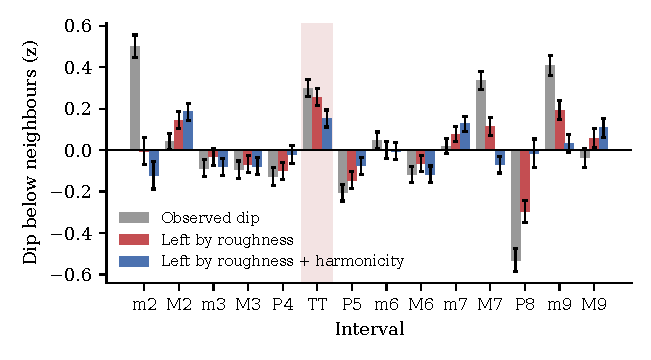
\includegraphics[width=0.66\linewidth]{figures/fig_null.pdf}
\caption{Dip of each integer interval below the mean of its two semitone neighbours, pooled
over eight US experiments with fixed-effect (inverse-variance) weights; bars, $\pm1.96$ pooled
SE. Grey: observed. Red: left by calibrated \HK{} roughness. Blue: left by roughness plus
harmonicity at the published 6.83-cent tolerance. Each interval's calibration excludes its
own window. Shaded: tritone.}
\label{fig:null}
\end{figure}

% =====================================================================
\section{The in-tune bonus and the step}
\label{sec:bonus}
All analyses in this section are exploratory; the patterns were noticed in the residual
profile. Three curves are compared: M1, \HK{} roughness plus harmonicity at 20 cents; M2, M1
plus a linear term in interval size (the curve used in the main text); M3, M1 plus the
sharpness proxy of Section~\ref{sec:sharpness}. For each, the held-out residual $r(c)$ is split
at each equal-tempered interval $c$ into a local bonus
$b(c)=r(c)-[r(c-0.5)+r(c+0.5)]/2$ and a baseline $q(c)=[r(c-0.5)+r(c+0.5)]/2$, so that
$r(c)=b(c)+q(c)$ and the gap $r(8)-r(6)$ splits into a bonus part $b(8)-b(6)$ and a baseline
part $q(8)-q(6)$. The step is the coefficient of an indicator for $c\ge8$ in a regression of
$q(c)$ on $c$ over 1--11 semitones (or 1--14), or the increment $q(8)-q(7)$ minus the mean of
the other increments.

\paragraph{Plain means and random effects.}
Table~\ref{tab:decompmodels} gives every quantity under both a plain mean over the six
harmonic spectra, with a participant-bootstrap CI that treats the spectra as fixed, and
random-effects pooling with a Hartung--Knapp CI, which treats them as a sample. The two
disagree. Under plain means the bonus part (M2: \decTwoBonusPartFixed), the baseline part
(\decTwoBasePartFixed), the step (\decTwoStepFixed) and the tritone's bonus shortfall relative
to the other intervals (\decTwoOtherMinusTTFixed) all exclude zero, as they do under M1 and
M3. Under random effects the bonus part (\decTwoBonusPart), the step as an indicator
(\decTwoStep) and the tritone's shortfall (\decTwoOtherMinusTT; M1 \decOneOtherMinusTT, M3
\decThreeOtherMinusTT) include zero, while the gap (\decTwoGap), the baseline part
(\decTwoBasePart) and the step as an increment (\decTwoStepInc) do not. The main text reports
the random-effects version, as for the primary estimand, because the question is about
spectra in general. The plain-mean figures answer a narrower question, about these six spectra,
and the statement in an earlier analysis by the author that the tritone receives about half the bonus rested on
them; it is withdrawn. The same plain-mean contrast computed on the curve with the sharpness
term (the version reported in that earlier analysis) is \gbSharpHarmDiff.

One contrast holds under both: the major second and minor seventh receive a smaller bonus
than the other eight intervals from the minor second to the major seventh (random effects
\decTwoMMvsRest; plain \decTwoMMvsRestFixed), and the tritone does not differ from them
(\decTwoTTvsMM). This contrast was chosen after seeing the profile. The individual bonuses
under M2 (plain means, point estimates) are \decTwoBMinSec, \decTwoBMajSec, \decTwoBMinThird,
\decTwoBMajThird, \decTwoBFourth, \decTwoBTritone, \decTwoBFifth, \decTwoBMinSixth,
\decTwoBMajSixth, \decTwoBMinSev{} and \decTwoBMajSev{} from the minor second to the major
seventh.

\paragraph{The step across analysis choices and spectra.}
Table~\ref{tab:step} repeats the step under M2 with other kernel widths, exclusion windows
and raw 0.25-semitone bins. The plain-mean step is stable across these choices (kernel SD 0.1:
\srStepSdOne; 0.3: \srStepSdThree; window $\pm0.4$: \srStepWinFour; $\pm0.8$: \srStepWinEight;
bins: \srStepBin), but in every variant it comes mainly from the guitar and piano, whose
spectra are proxies from one analysed tone each, and it is absent for the synthetic harmonic
tone and the flute.

\begin{table}[h]
\centering
\caption{Decomposition of the held-out gap under three curves (exploratory). For each: plain
mean over the six harmonic spectra [participant-bootstrap CI] and random effects
[Hartung--Knapp CI]. M1: \HK{} + harmonicity (20 cents); M2: + interval size; M3: + sharpness
proxy. Bold: CI excludes zero.}
\label{tab:decompmodels}
\scriptsize
\setlength{\tabcolsep}{2pt}
\resizebox{\linewidth}{!}{%
\begin{tabular}{lcccccc}
\toprule
& \multicolumn{2}{c}{M1} & \multicolumn{2}{c}{M2} & \multicolumn{2}{c}{M3} \\
\cmidrule(lr){2-3}\cmidrule(lr){4-5}\cmidrule(lr){6-7}
Quantity & Plain & Random effects & Plain & Random effects & Plain & Random effects \\
\midrule
\tabinput{tables/tab_supp_decomp_models.tex}
\bottomrule
\end{tabular}}
\end{table}

\begin{table}[h]
\centering
\caption{The step (M2) under other analysis choices (exploratory): plain mean over the six
harmonic spectra [participant-bootstrap CI] of the step as an indicator and as an increment,
the bonus and baseline parts of the gap, and the step per spectrum (point estimates). Guitar
and piano use proxy spectra. Bold: CI excludes zero.}
\label{tab:step}
\scriptsize
\setlength{\tabcolsep}{2pt}
\resizebox{\linewidth}{!}{%
\begin{tabular}{lcccccccccc}
\toprule
& \multicolumn{4}{c}{Six harmonic spectra} & \multicolumn{6}{c}{Step per spectrum} \\
\cmidrule(lr){2-5}\cmidrule(lr){6-11}
Variant & Step & Increment & Bonus part & Baseline part & Harm. & 5 eq. & No 3rd & Flute & Guitar & Piano \\
\midrule
\tabinput{tables/tab_supp_step.tex}
\bottomrule
\end{tabular}}
\end{table}

% =====================================================================
\section{Stretched and compressed partials}
\label{sec:stretched}

\paragraph{The dip at the stretched scale.}
Repeating the analysis at the stretched scale's own fourth, tritone, fifth and minor sixth,
the stretched tones show an observed dip of \sscObsDipStr{} at \sscPosStr{} semitones (paired
difference from the dip at 6, on the same bootstrap draws, \sscObsDipStrDiff). Calibrated \HK{}
roughness fitted to the stretched experiment itself leaves \sscHKDipStr{} of it, and adding
harmonicity changes little (\sscHKHDipStr). The gap to the stretched minor sixth is
\sscObsGapStr. For compressed tones the dip at \sscPosComp{} is \sscObsDipComp{} (paired
difference \sscObsDipCompDiff). For harmonic tones the procedure returns the ordinary
estimates (dip \sscObsDipHarm).

\paragraph{The bonus at the stretched scale (A4).}
If the in-tune bonus were attached to intervals as heard relative to the heard octave, it
should appear at the stretched scale's own intervals. Table~\ref{tab:strbonus} gives the mean
bonus of the intervals other than the tritone at the scale matched to each spectrum and at the
equal-tempered positions, with the minimum effect detectable with 80\% power (2.8 SE). For US
listeners the bonus is \sbOwnHarm{} for harmonic tones and \sbOwnStr{} and \sbOwnComp{} at the
stretched and compressed scales, with detectable effects of \sbMdeStr{} and \sbMdeComp. The
absence is therefore not a matter of power.

\begin{table}[h]
\centering
\caption{Mean in-tune bonus of the intervals other than the tritone (exploratory; M2 curve)
at the scale matched to each spectrum and at equal-tempered positions [participant-bootstrap
CI], and the minimum detectable effect (MDE, 2.8 SE). Bold: CI excludes zero.}
\label{tab:strbonus}
\footnotesize
\begin{tabular}{lccc}
\toprule
Spectrum (cohort) & Own scale & Equal-tempered & MDE \\
\midrule
\tabinput{tables/tab_supp_strbonus.tex}
\bottomrule
\end{tabular}
\end{table}

\paragraph{Timbre-relative harmonicity.}
\label{sec:timbrerel}
The published harmonicity model cannot follow the shifted dip, because its template is a
harmonic series. As an exploratory step taken after the screen, we replaced the template with
the upper tone's own partials and let the pitch-class circle wrap at the tone's own octave,
one way of reading the proposal that harmonic templates are learned from the sounds heard
\citep{shamma2000}. Out of sample, this model predicts a dip of \mbStrPredSelf{} at
\sscPosStr{} semitones for the stretched tones and leaves \mbStrSscSelf{} \mbStrSscSelfCI,
against \mbStrSscHKH{} \mbStrSscHKHCI{} with the standard template (paired difference
\mdStrSscSelfVsHKH); Marjieh et al.'s revised roughness also leaves little there
(\mbStrSscRev). With one stretched experiment neither residual is distinguishable from zero.
The model pays for this on harmonic tones: the dip left at 600 cents rises to \mbDipSelf{}
(standard template \mbDipHKH; paired difference \mdDipSelfVsHKH) and the held-out $R^2$ falls
to \mbRtwoSelf{} (paired difference \mdRtwoSelfVsHKH). Adding it to the 20-cent term does not
improve the fit (paired $R^2$ difference \mdRtwoTwSelfVsTw). In summary, a template matched to
the timbre can reproduce the stretched-scale dip but is not a better general curve, and a
single stretched spectrum cannot decide between it and revised roughness.

% =====================================================================
\section{Roll-off}
\label{sec:rolloff}
Table~\ref{tab:rolloff} gives the roll-off experiment at the three pre-set roll-off levels.
The roughness curve predicts almost no gap at any roll-off, and the observed gap does not
shrink as the upper partials fade.

\begin{table}[h]
\centering
\caption{Study~3 of \citet{marjieh2024} (harmonic tones, roll-off varied continuously;
$N=\nRoll$), smoothed at three roll-off levels (kernel SD 1.5\,dB/octave). Pred.: gap predicted
by the calibrated roughness curve. SD units [95\% CI]. Bold: CI excludes zero.}
\label{tab:rolloff}
\footnotesize
\setlength{\tabcolsep}{4pt}
\resizebox{\linewidth}{!}{%
\begin{tabular}{lcccccc}
\toprule
dB/oct & Observed gap & Roughness pred. & After roughness & After rough.\ + harm. & Observed dip & Dip after rough.\ + harm. \\
\midrule
\tabinput{tables/tab_rolloff.tex}
\bottomrule
\end{tabular}}
\end{table}

% =====================================================================
\section{Korean listeners}
\label{sec:korean}
Korean listeners rating the same harmonic stimuli show a smaller gap than US listeners
(difference \cohObsGapHarm; after roughness and harmonicity \cohHKHGapHarm). Their dip at the
tritone is clear (\dipObsHarmKr{} \dipObsHarmKrCI) and the two-mechanism curve accounts for it
(\dipHKHHarmKr). The cohort difference is not specific to harmonic tones: Korean listeners also
rate the minor sixth lower relative to the tritone for stretched (\cohObsGapStr) and compressed
(\cohObsGapComp) partials, where US listeners show no gap.

\paragraph{In-sample fits.}
Fitted to each Korean experiment alone (in-sample), roughness plus harmonicity at 20 cents
reaches $R^2$ of \insBaseKRmin--\insBaseKRmax; adding a linear term in interval size raises
the mean to \insXKR, and adding the sharpness proxy instead raises the range to
\insSharpKRmin--\insSharpKRmax, close to but below the split-half ceilings (\krCeilMin--\krCeilMax). These in-sample figures overstate what the
models predict.

\paragraph{Held-out fits (A3).}
Table~\ref{tab:korean} predicts the Korean experiments with weights fitted to all US
experiments. The recommended curve does worse than each experiment's mean (mean held-out $R^2$
\krHoTw), as does the composite (\krHoComp); a linear term in interval size brings the mean to
\krHoSize{} and the sharpness proxy to \krHoSharp. What the curves miss for Korean listeners
is mainly a steeper decline of pleasantness with interval size. Sharpness is one candidate
cause; in an online study, differences in playback equipment between cohorts are another.

\begin{table}[h]
\centering
\caption{Korean experiments predicted with weights from US listeners (exploratory): held-out
$R^2$ [participant-bootstrap CI], and the split-half ceiling.}
\label{tab:korean}
\footnotesize
\setlength{\tabcolsep}{3pt}
\resizebox{\linewidth}{!}{%
\begin{tabular}{lcccc}
\toprule
Model & Harmonic & Stretched 2.1 & Compressed 1.9 & Mean \\
\midrule
\tabinput{tables/tab_supp_korean.tex}
\bottomrule
\end{tabular}}
\end{table}

% =====================================================================
\section{The smooth trend and the sharpness proxy}
\label{sec:sharpness}
All analyses in this section are exploratory, except the triad test, whose predictions were
written down before the triad data were read.

\paragraph{The proxy.}
$S$ is the loudness-weighted mean critical-band rate of the partials (weights
amplitude$^{0.6}$) with Zwicker's high-frequency weighting, $g(z)=1$ below 15.8\,Bark and
$0.066\,e^{0.171z}$ above \citep{zwicker2007}. It is computed from the synthesis parameters, not
from audio, and is not a calibrated sharpness in acum. It was chosen over interval size and
the log spectral centroid by the same held-out criterion that we report, so its advantage over
them is optimistic.

\paragraph{Pooled weights.}
Pooling all ten US experiments, the three-term curve with the 20-cent harmonicity tolerance
has weights $b_R=\shBetaR$, $b_H=\shBetaH$ and $b_S=\shBetaS$ per unit of $S$ (weighted Bark),
in the units of the two-term curve of main-text Section~\ref{M-sec:curve}. We do not
propose it as the recommended curve, because the proxy was chosen after seeing the residuals
and failed its pre-specified test (Section~\ref{sec:triadtest}).

\paragraph{The roll-off check.}
Fitted separately at five roll-offs (kernel SD 1.5\,dB/octave), the slope over interval size of
the residual after roughness and harmonicity flattens as the roll-off steepens
(Table~\ref{tab:roslope}; difference between 1 and 13\,dB/octave \roSlopeDiff). With one weight
shared across roll-offs, sharpness fits better than interval size (mean $R^2$ \roSharpRtwo{}
against \roXRtwo; difference \roSharpMinusX; roughness and harmonicity alone \roBaseRtwo), but
the slopes it implies cover only about \roImpShare\% of the observed flattening. The two terms
are strongly correlated, so the sign of the interval-size term with both in the model
(\roXSharpBetaX{} per octave; sharpness \roXSharpBetaS) is weak evidence. We looked at this
experiment before choosing sharpness, so it motivated the hypothesis as much as it tests it.

\begin{table}[h]
\centering
\caption{Roll-off experiment (exploratory): slope over interval size of the residual after
\HK{} roughness plus harmonicity (20 cents), SD per octave of interval [participant-bootstrap
CI], and the slope implied by the sharpness proxy with one shared weight.}
\label{tab:roslope}
\footnotesize
\begin{tabular}{lcc}
\toprule
Roll-off (dB/octave) & Observed slope & Implied by sharpness \\
\midrule
1 & \roSlopeOne & \roImpOne \\
4 & \roSlopeFour & \roImpFour \\
7 & \roSlopeSeven & \roImpSeven \\
10 & \roSlopeTen & \roImpTen \\
13 & \roSlopeThirteen & \roImpThirteen \\
\bottomrule
\end{tabular}
\end{table}

\paragraph{The pre-specified triad test.}
\label{sec:triadtest}
Before reading them, we wrote down (but did not publicly register) three predictions for the one rating set of Marjieh et al.\
not yet analysed: \ctNChords{} triads of five equal harmonics with and without the third
harmonic, rated by \ctNPart{} participants. Fitted to the triads, the sharpness weight should be
negative; adding sharpness should improve leave-one-chord-out $R^2$; and the three-term curve
with frozen dyad weights should correlate better with the chord means than the two-term curve.
We also recorded the risk that the trend had been absent for five equal harmonics in the dyads.
None of the three predictions passed. The fitted weight was negative but its interval included
zero (\ctBS); leave-one-chord-out $R^2$ went from \ctLooTwo{} to \ctLooThree{} (\ctLooDiff); and
the frozen-weight correlation went from \ctRTwo{} to \ctRThree{} (\ctRDiff). The triads leave little
room for a third term, but they do not confirm it.

% =====================================================================
\section{Equal temperament and just intonation (A8)}
\label{sec:etji}
This analysis is exploratory; it was added after the dense-dyad residuals had been seen. It
asks whether evaluating the gap at equal-tempered positions creates part of it. With a kernel
of SD 0.1 semitones (sensitivity: 0.05 and 0.2), we located, per experiment with a
participant-bootstrap CI, the listeners' minor-sixth peak (argmax over 7.5--8.5 semitones),
tritone trough (argmin over 5.5--6.5) and, as controls, the peaks of the fifth, major third and
major sixth, on the listener profile and on the held-out predictions of each model
(Table~\ref{tab:etjiloc}, Figure~\ref{fig:etji}). We then recomputed the gap at equal-tempered
positions and at two just-intoned pairs: 8/5 against 7/5 (JIa) and 8/5 against 45/32 (JIb)
(Table~\ref{tab:etjigap}).

Pooled over the six harmonic spectra, the listeners' minor-sixth peak lies at \ejLocMsix{}
cents, \ejDiffMsix{} cents from the peak of the harmonicity model at the published tolerance
(\ejModelMsix); at the narrower width it is \ejLocMsixNarrow{} (difference
\ejDiffMsixNarrow). The fifth peaks where the model does (\ejDiffPfive), and the major third
and major sixth lie \ejDiffMThree{} and \ejDiffMajSix{} cents from the model's peaks, each
displaced from the model's just-intoned peak towards equal temperament, as the minor sixth is,
but none of these differences is established. The tritone
region is a broad trough (\ejLocTT) with no distinct minimum at 600 cents or at either
just-intoned tritone. The gap left by the recommended curve is \ejGapET{} at equal-tempered
positions and \ejGapJIa{} and \ejGapJIb{} at the just-intoned pairs; the paired differences,
\ejGapJIaDiff{} and \ejGapJIbDiff, show neither a smaller gap at just intonation nor
equivalence within $\pm0.05$\SDu. The result is inconclusive. The recommended curve has no
interior minor-sixth or major-third peak at this width (rows marked ``edge''), so it smooths
away a peak that listeners show.

\begin{table}[h]
\centering
\caption{Peak and trough locations (cents) [participant-bootstrap CI; pooled rows, random
effects with Hartung--Knapp CI], kernel SD 0.1 semitones (exploratory). Equal-tempered and
just-intoned positions: m6 800/814; TT 600/583 (7/5) or 590 (45/32); P5 700/702; M3 400/386;
M6 900/884. $^\dagger$Point estimate on the edge of the search window. Edge: extremum on the
window edge in at least one spectrum.}
\label{tab:etjiloc}
\scriptsize
\setlength{\tabcolsep}{3pt}
\resizebox{\linewidth}{!}{%
\begin{tabular}{lccccc}
\toprule
& m6 peak & TT trough & P5 peak & M3 peak & M6 peak \\
\midrule
\tabinput{tables/tab_supp_etji_loc.tex}
\bottomrule
\end{tabular}}
\end{table}

\begin{table}[h]
\centering
\caption{Gap at equal-tempered (ET) and just-intoned positions (JIa: 8/5 vs 7/5; JIb: 8/5 vs
45/32), observed and left by each held-out model, random effects over the six harmonic spectra
[Hartung--Knapp CI], at three kernel widths (semitones; exploratory). A kernel of 0.2
semitones cannot separate positions 14 cents apart.}
\label{tab:etjigap}
\scriptsize
\setlength{\tabcolsep}{2.5pt}
\resizebox{\linewidth}{!}{%
\begin{tabular}{llccccc}
\toprule
SD & & ET & JIa & JIb & JIa $-$ ET & JIb $-$ ET \\
\midrule
\tabinput{tables/tab_supp_etji_gap.tex}
\bottomrule
\end{tabular}}
\end{table}

\begin{figure}[h]
\centering
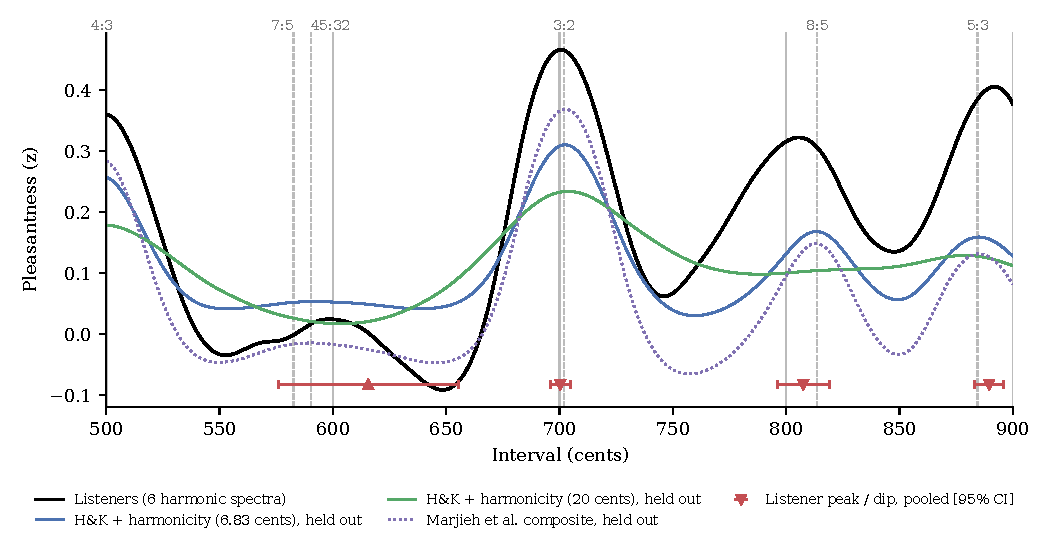
\includegraphics[width=\linewidth]{figures/fig_etji.pdf}
\caption{Pooled listener profile of the six harmonic spectra at kernel SD 0.1 semitones
(black) with the held-out model curves, from 500 to 900 cents (exploratory). Solid grey
lines: equal-tempered positions; dashed: just-intoned ratios. Red markers: pooled listener
peak and trough locations [Hartung--Knapp CI].}
\label{fig:etji}
\end{figure}

% =====================================================================
\section{Chords: the three-component decomposition}
\label{sec:chorddecomp}
Table~\ref{tab:chorddecomp} and Figure~\ref{fig:chorddecomp} give the unique variance of
interference (\HK), harmonicity and familiarity, each over the other two, in the Bowling and
Johnson-Laird chords under four covariate specifications. With chord size controlled and
equal-tempered scoring, the unique variance of harmonicity in the Bowling chords
(\dRBSizeH) was about half that of interference (\dRBSizeI) and familiarity (\dRBSizeF). Scored
at the just intonation actually presented, the three are comparable (\dRBjiSizeI, \dRBjiSizeH{}
and \dRBjiSizeF), and the full model's $R^2$ rises from \RfullBSize{} to \RfullBjiSize. Without
a chord-size control familiarity appears to dominate (\dRBRawF{} against \dRBRawI{} for
interference), which is how an earlier analysis by the author reported it. Across the 298
chords, harmonicity scored in the two tunings correlates $r=\rEtJiH$. The chord bootstraps
resample chords, not raters.

\begin{table}[h]
\centering
\caption{Unique $\Delta R^2$ [95\% bootstrap CI] ($p$, nested $F$) of interference (\HK),
harmonicity and familiarity over the other two, under four covariate specifications. $R^2$:
full model including covariates.}
\label{tab:chorddecomp}
\footnotesize
\setlength{\tabcolsep}{4pt}
\resizebox{\linewidth}{!}{%
\begin{tabular}{lrccc}
\toprule
Covariates & $R^2$ & Interference & Harmonicity & Familiarity \\
\midrule
\tabinput{tables/tab_decomp.tex}
\bottomrule
\end{tabular}}
\end{table}

\begin{figure}[h]
\centering
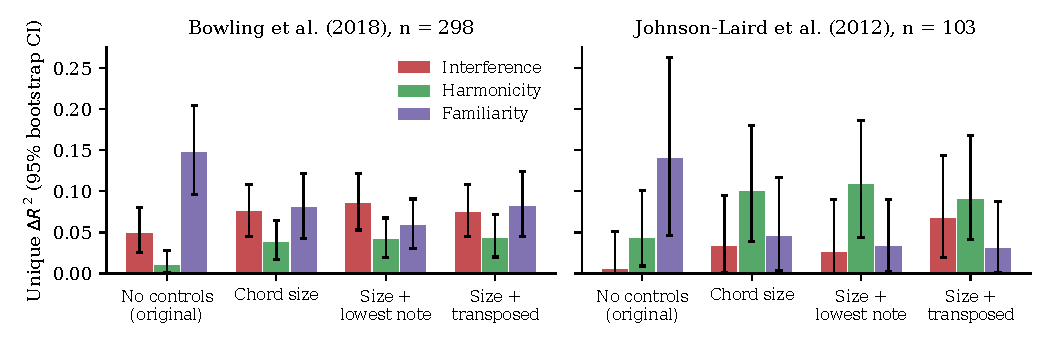
\includegraphics[width=\linewidth]{figures/fig5_decomposition.pdf}
\caption{Unique $\Delta R^2$ of interference, harmonicity and familiarity (95\% bootstrap CI)
under four covariate specifications, models scored in equal temperament.}
\label{fig:chorddecomp}
\end{figure}

% =====================================================================
\section{Roughness curves on measured spectra}
\label{sec:measured}
Could the problem lie in idealised spectra? A dissonance curve computed from a measured
spectrum might place the tritone above the minor sixth. We computed the tritone/minor-sixth
roughness difference, $(D_{600}-D_{800})/D_{800}$, for \nMeasuredSpectra{} measured spectra
under four roughness kernels (Sethares with product and minimum weighting, Vassilakis and
\HK). The answer depends on the analysis more than on anything a listener would recognise
(Table~\ref{tab:gaps}, Figure~\ref{fig:gaps}). On one Philharmonia clarinet spectrum the four
kernels give \gapClarCFourHK, \gapClarCFourS, \gapClarCFourSmin{} and \gapClarCFourV\%, a range
of \rangeClarKernels\pp. Across the eight C4 instruments the instrument accounts for
\shareInstrNoV\% of the variance of the difference, the kernel for \shareModelNoV\% and their
interaction for \shareInterNoV\% (three stable kernels). The shape constants of the \HK{}
kernel, which are rarely reported, move the difference by a median \sensABNarrowMed\pp{} over
a $\pm$20\% grid, and the recording (two clarinet libraries) by a median
\sensRecordingMed\pp{} (Table~\ref{tab:sens}, Figure~\ref{fig:sens}).

One ordering is robust: under \HK{} the clarinet rates the minor sixth rougher than the tritone
at three registers in both libraries (Iowa: \iowaHKDThree, \iowaHKCFour{} and \iowaHKCFive\%;
Table~\ref{tab:gapsreg}, Figure~\ref{fig:curves}). The reversal comes from a single pair of odd
harmonics at the minor sixth (the fifth of the lower note against the third of the upper,
\mechHKpairBeat\,Hz apart, \mechHKpairShare\% of cross-tone roughness) and from the steep decay
of the \HK{} kernel beyond its peak (Figure~\ref{fig:mech}). Depending on instrument and kernel,
roughness computed from real spectra can reverse the listeners' ordering as easily as
reproduce it.

\paragraph{Extraction.}
Sustained forte notes were taken from the Philharmonia library \citep{philharmonia}: cello,
clarinet, oboe, flute, bassoon, saxophone and French horn at C4, plus low and high registers
for clarinet (D3, C5), cello (C3, C5) and oboe (A\sh3, C5); a piano C4 and three further
clarinet notes (D3, C4, C5) came from the Iowa library \citep{iowamis}. Each note was analysed
with an 8192-point STFT (75\% overlap) over the stable middle 60\% of the sample. Peaks with
prominence above $0.005$ of the loudest partial were accepted and the 15 strongest kept;
frequencies were refined by parabolic interpolation on log magnitude. The Iowa piano's
partials follow the stiff-string law $f_n=nf_0\sqrt{1+Bn^2}$ \citep{fletcher1964} with
$B=\pianoB\times10^{-4}$ (SE $\pianoBse\times10^{-7}$).

\paragraph{Kernels.}
Sethares (product): $e^{-3.5s\Delta f}-e^{-5.75s\Delta f}$ with
$s=0.24/(0.0207f_{\min}+18.96)$, weighted by $a_1a_2$ \citep{sethares1993,sethmatlab};
Sethares (min): weighted by $\min(a_1,a_2)$ \citep{sethares2005}; Vassilakis: weighted by
$(a_1a_2)^{0.1}(2\min(a_1,a_2)/(a_1+a_2))^{3.11}$ \citep{vassilakis2001}; \HK{} as in main-text
Section~\ref{M-sec:models}; as a sensitivity check the ERB of \citet{glasberg1990} replaced
the critical bandwidth. Coincident partials were merged in
quadrature. Each spectrum's dyad was swept from unison to the octave in 5-cent steps.
Implementations differ between packages \citep{mashinter2006}.

\paragraph{Sensitivity factors.}
Instrument (eight at C4); kernel; \HK{} constants on a wide grid, $a$ = \abGridA{} crossed with
$b$ = \abGridB, and on a narrow grid, $a$ = 0.2, 0.25, 0.3 crossed with $b$ = 1.5, 2, 2.5;
recording (Philharmonia vs Iowa clarinet); extraction constants (prominence $0.005$--$0.0002$,
cap 15 or 25); audio codec (lossless to 48\,kbit/s MP3); idealised-spectrum constants (5, 7 or
11 harmonics, roll-off 0.8--1.0). Under the narrow grid the sign of the \HK{} difference is
stable for \abStableNarrow{} of \abNSpectra{} spectra. Vassilakis's near-flat amplitude weight
makes it depend on how many weak partials are admitted (extraction moves it by up to
\sensVassExtractMax\pp; Table~\ref{tab:vassexp}).

\paragraph{Clarinet.}
Table~\ref{tab:clarinet} tests the \HK{} clarinet reversal against every constant. It survives
the extraction sweep (range at most \clarHKExtrMax\pp), the cutoff sweep, ERB substitution and
the whole narrow $a,b$ grid on both libraries (Table~\ref{tab:supphk}). At the minor sixth the
fifth harmonic of the lower note (\mechHKpairFlo\,Hz) and the third of the upper
(\mechHKpairFhi\,Hz) lie near the peak of the \HK{} kernel; at the tritone the fundamentals are
\mechFundCBW{} critical bandwidths apart, where the \HK{} weight is \mechFundGpct\% of its peak
but the Sethares kernel still assigns substantial roughness (\mechSethFundShare\% of its
cross-tone total). Listener ratings of clarinet dyads at several registers would discriminate
between kernels.

\begin{table}[h]
\centering
\caption{Tritone/minor-sixth roughness difference (\%) at C4. Bold: negative (the kernel rates
the minor sixth rougher). Vassilakis values are highly sensitive to extraction settings and
should be read for sign only.}
\label{tab:gaps}
\small
\begin{tabular}{lrrrr}
\toprule
Spectrum & Sethares & Sethares-min & Vassilakis & \HK \\
\midrule
\tabinput{tables/tab_gaps_c4.tex}
\bottomrule
\end{tabular}
\end{table}

\begin{table}[h]
\centering
\caption{Tritone/minor-sixth roughness difference (\%) at three registers (Philharmonia).
Bold: negative.}
\label{tab:gapsreg}
\small
\begin{tabular}{lrrrr}
\toprule
Spectrum & Sethares & Sethares-min & Vassilakis & \HK \\
\midrule
\tabinput{tables/tab_gaps_register.tex}
\bottomrule
\end{tabular}
\end{table}

\begin{table}[h]
\centering
\caption{Range of the tritone/minor-sixth roughness difference (pp) across the levels of each
analysis factor. $n$: number of (spectrum, kernel) cells for the three stable kernels. For the
instrument row each cell is one kernel across the eight C4 instruments. $^\dagger$\HK{} only.
$^\ddagger$For Vassilakis this row shows its amplitude exponent varied over
$\{0.1,0.25,0.5,1\}$.}
\label{tab:sens}
\small
\begin{tabular}{lrrrrr}
\toprule
& & \multicolumn{2}{c}{Stable kernels} & \multicolumn{2}{c}{Vassilakis} \\
\cmidrule(lr){3-4}\cmidrule(lr){5-6}
Factor & $n$ & Median & Max & Median & Max \\
\midrule
\tabinput{tables/tab_sensitivity.tex}
\bottomrule
\end{tabular}
\end{table}

\begin{table}[h]
\centering
\caption{Robustness of the \HK{} clarinet difference (\%). Extraction: range (pp) across the
extraction sweep. Cutoff: range with the 1.2-CBW cutoff at 1.2, 1.5, 2.0 or removed
(Philharmonia only). Narrow/wide: range over the $a,b$ grids. ERB: difference with the ERB in
place of the CBW. Bold: positive.}
\label{tab:clarinet}
\small
\resizebox{\linewidth}{!}{%
\begin{tabular}{llrrcccr}
\toprule
Reg. & Library & Diff. & Extraction & Cutoff & Narrow $a,b$ & Wide $a,b$ & ERB \\
\midrule
\tabinput{tables/tab_clarinet.tex}
\bottomrule
\end{tabular}}
\end{table}

\begin{table}[h]
\centering
\caption{\HK{} tritone/minor-sixth difference (\%) per spectrum under the $a,b$ grids and ERB
substitution. Bold: sign differs from the baseline.}
\label{tab:supphk}
\small
\begin{tabular}{lrccrr}
\toprule
Spectrum & Baseline & Narrow $a,b$ & Wide $a,b$ & ERB, cut 1.2 & ERB, no cut \\
\midrule
\tabinput{tables/tab_supp_hk.tex}
\bottomrule
\end{tabular}
\end{table}

\begin{table}[h]
\centering
\caption{Vassilakis tritone/minor-sixth difference (\%) as the amplitude exponent varies
(published value 0.1). Bold: sign differs from the published-exponent value.}
\label{tab:vassexp}
\small
\begin{tabular}{lrrrr}
\toprule
Spectrum & 0.1 & 0.25 & 0.5 & 1.0 \\
\midrule
\tabinput{tables/tab_supp_vass.tex}
\bottomrule
\end{tabular}
\end{table}

\begin{figure}[h]
\centering
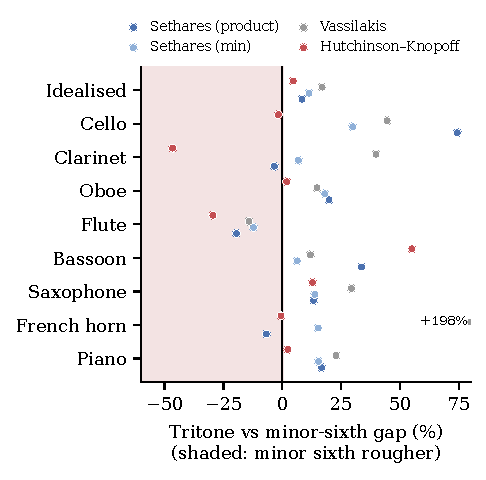
\includegraphics[width=0.7\linewidth]{figures/fig1_gaps.pdf}
\caption{Tritone/minor-sixth roughness difference (\%) per spectrum and kernel at C4 (shaded:
the kernel rates the minor sixth rougher).}
\label{fig:gaps}
\end{figure}

\begin{figure}[h]
\centering
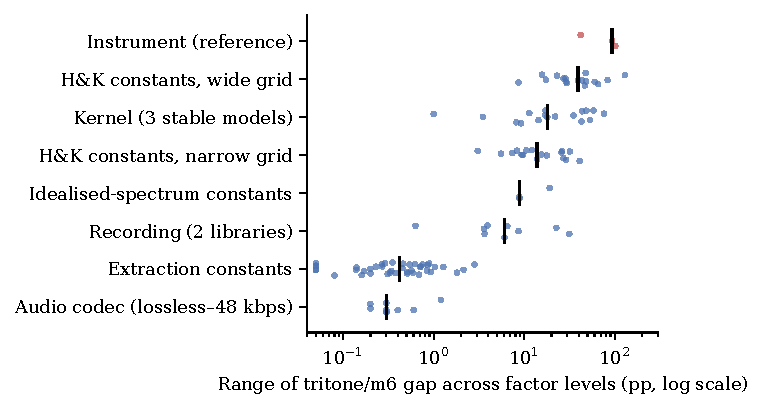
\includegraphics[width=0.75\linewidth]{figures/fig2_sensitivity.pdf}
\caption{Range of the tritone/minor-sixth difference (pp, log scale) across the levels of each
analysis factor, stable kernels; bars, medians. Red: instrument (reference).}
\label{fig:sens}
\end{figure}

\begin{figure}[h]
\centering
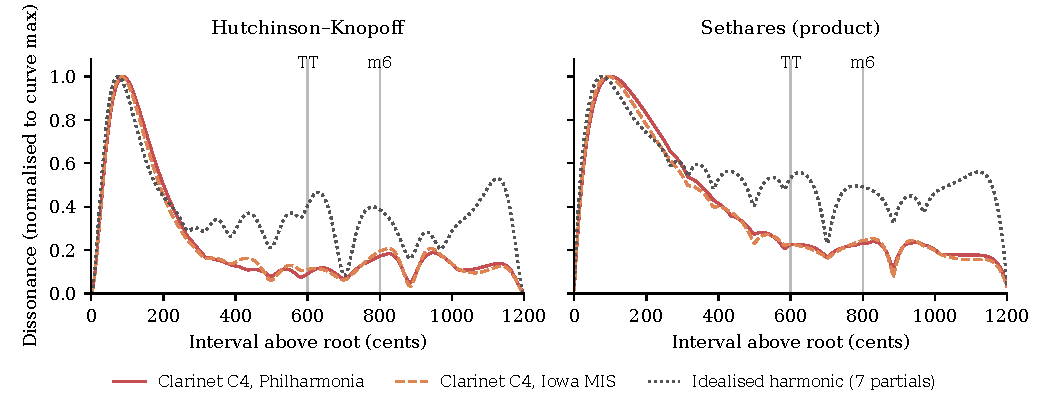
\includegraphics[width=\linewidth]{figures/fig3_curves.pdf}
\caption{Dissonance curves (normalised to each curve's maximum) for two clarinet C4 recordings
and an idealised seven-partial harmonic tone, under the \HK{} and Sethares (product) kernels.}
\label{fig:curves}
\end{figure}

\begin{figure}[h]
\centering
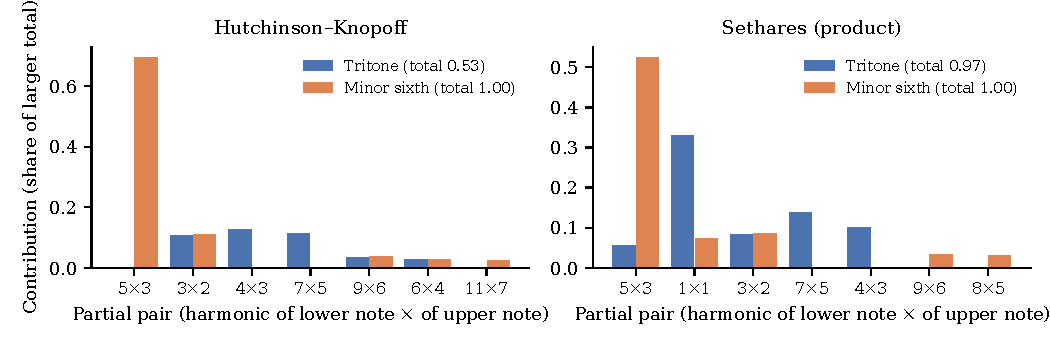
\includegraphics[width=\linewidth]{figures/fig4_mechanism.pdf}
\caption{Philharmonia clarinet C4: the partial pairs contributing most roughness at the
tritone and the minor sixth under each kernel (share of the larger total).}
\label{fig:mech}
\end{figure}

% Generated by analysis/apa_refs.py from refs.bib (APA 7). Do not edit by hand.
\begin{thebibliography}{12}
\bibitem[{Fastl \apaand{} Zwicker(2007)Fastl and Zwicker}]{zwicker2007}
Fastl, H., \& Zwicker, E. (2007). \emph{Psychoacoustics: Facts and models} (3rd ed.). Springer. \url{https://doi.org/10.1007/978-3-540-68888-4}

\bibitem[{Fletcher(1964)Fletcher}]{fletcher1964}
Fletcher, H. (1964). Normal vibration frequencies of a stiff piano string. \emph{The Journal of the Acoustical Society of America}, \emph{36}(1), 203--209. \url{https://doi.org/10.1121/1.1918933}

\bibitem[{Glasberg \apaand{} Moore(1990)Glasberg and Moore}]{glasberg1990}
Glasberg, B. R., \& Moore, B. C. J. (1990). Derivation of auditory filter shapes from notched-noise data. \emph{Hearing Research}, \emph{47}(1--2), 103--138. \url{https://doi.org/10.1016/0378-5955(90)90170-T}

\bibitem[{Marjieh et~al.(2024)Marjieh, Harrison, Lee, Deligiannaki, and Jacoby}]{marjieh2024}
Marjieh, R., Harrison, P. M. C., Lee, H., Deligiannaki, F., \& Jacoby, N. (2024). Timbral effects on consonance disentangle psychoacoustic mechanisms and suggest perceptual origins for musical scales. \emph{Nature Communications}, \emph{15}, 1482. \url{https://doi.org/10.1038/s41467-024-45812-z}

\bibitem[{Mashinter(2006)Mashinter}]{mashinter2006}
Mashinter, K. (2006). Calculating sensory dissonance: Some discrepancies arising from the models of Kameoka \& Kuriyagawa, and Hutchinson \& Knopoff. \emph{Empirical Musicology Review}, \emph{1}(2), 65--84. \url{https://doi.org/10.18061/1811/24077}

\bibitem[{Philharmonia Orchestra(n.d.)Philharmonia Orchestra}]{philharmonia}
Philharmonia Orchestra. (n.d.). \emph{Sound samples}. Retrieved August 2026, from \url{https://philharmonia.co.uk/resources/sound-samples/}

\bibitem[{Schlecht(2020)Schlecht}]{sethmatlab}
Schlecht, S. J. (2020). \emph{dissonanceSethares: MATLAB implementation of Sethares' dissonance measure} [Computer software]. \url{https://github.com/SebastianJiroSchlecht/dissonanceSethares}

\bibitem[{Sethares(1993)Sethares}]{sethares1993}
Sethares, W. A. (1993). Local consonance and the relationship between timbre and scale. \emph{The Journal of the Acoustical Society of America}, \emph{94}(3), 1218--1228. \url{https://doi.org/10.1121/1.408175}

\bibitem[{Sethares(2005)Sethares}]{sethares2005}
Sethares, W. A. (2005). \emph{Tuning, timbre, spectrum, scale} (2nd ed.). Springer. \url{https://doi.org/10.1007/b138848}

\bibitem[{Shamma \apaand{} Klein(2000)Shamma and Klein}]{shamma2000}
Shamma, S., \& Klein, D. (2000). The case of the missing pitch templates: How harmonic templates emerge in the early auditory system. \emph{The Journal of the Acoustical Society of America}, \emph{107}(5), 2631--2644. \url{https://doi.org/10.1121/1.428649}

\bibitem[{University of Iowa Electronic Music Studios(n.d.)University of Iowa Electronic Music Studios}]{iowamis}
University of Iowa Electronic Music Studios. (n.d.). \emph{Musical instrument samples}. Retrieved August 2026, from \url{https://theremin.music.uiowa.edu/MIS.html}

\bibitem[{Vassilakis(2001)Vassilakis}]{vassilakis2001}
Vassilakis, P. N. (2001). \emph{Perceptual and physical properties of amplitude fluctuation and their musical significance} [Doctoral dissertation, University of California, Los Angeles].

\end{thebibliography}


\end{document}
